%++++++++++++++++++++++++++++++++++++++++
% Don't modify this section unless you know what you're doing!
\documentclass[letterpaper,10pt]{article}
\usepackage{blindtext}
\usepackage{authblk}
\usepackage{tabularx} % extra features for tabular environment
\usepackage{textcomp}
\usepackage{gensymb}
\usepackage{amsmath}  % improve math presentation
\usepackage{graphicx} % takes care of graphic including machinery
\usepackage{subfig}
\usepackage{wrapfig}
\usepackage{xcolor}
\usepackage{rotating}
\usepackage[margin=1in,letterpaper]{geometry} % decreases margins
\usepackage{setspace}
\usepackage{cite} % takes care of citations
\usepackage[final]{hyperref} % adds hyper links inside the generated pdf file
\hypersetup{
	colorlinks=true,       % false: boxed links; true: colored links
	linkcolor=blue,        % color of internal links
	citecolor=blue,        % color of links to bibliography
	filecolor=magenta,     % color of file links
	urlcolor=blue
}
%++++++++++++++++++++++++++++++++++++++++
\graphicspath{ {../plots/} }



\begin{document}

%--------------------------------------------------------------------------
%TITLE PAGE
%--------------------------------------------------------------------------

\doublespacing
\begin{center}
	\huge Imaging elastodynamic and hydraulic properties of in-situ fractured rock: An experimental investigation exploring effects of dynamic stressing and shearing

	\quad

	\large Journal: JGR: Solid Earth

	\quad

	\large Clay Wood, Parisa Shokouhi, Prabhakaran Manogharan, Jacques Rivi\`{e}re, Derek Elsworth, Chris Marone \\
	\large Acknowledge: Jiang Jin, Benjamin Madara

\end{center}
\clearpage




%--------------------------------------------------------------------------
%ABSTRACT
%--------------------------------------------------------------------------

\section{Abstract}
\paragraph{}
We describe laboratory work to elucidate the relationship between nonlinear elasticity and permeability evolution in fractured media subjected to local stress perturbations. This study is part of an effort to image fluid pathways and fracture properties using active-source acoustic monitoring during fluid injection and shear of rough fractures. Experiments were conducted in which intact L-shaped Westerly Granite samples were fractured in-situ under tri-axial conditions while forcing deionized water through the subsequent fracture interfaces. After in-situ fracturing, we imposed oscillations of the applied normal stress and pore pressure with amplitudes ranging from 0.2 to 1 MPa and frequencies from 0.1 to 40 Hz. During these dynamic perturbations an array of piezoelectric transducers continuously transmitted ultrasonic pulses across the fracture to monitor the elastic response. We interpret the resulting evolution of elastic wave properties in the context of elastic nonlinearity and relate the estimated nonlinearity parameters to the relative change in permeability of the fractured media. Further, fracture roughness is altered in-situ by shearing the L-shaped samples, which generates breccia and wear materials. We document the evolution of permeability and fracture contact stiffness as a function of dynamic stressing and shear offset and discuss our findings in relation to fractures in Earth's crust.
\clearpage



%--------------------------------------------------------------------------
%INTRODUCTION
%--------------------------------------------------------------------------

\section{Introduction}
\paragraph{} Dynamic stresses associated with energy production and waste water sequestration (injection, pumping, and transport of supercritical $H_{2}O$--$CO_{2}$ fluids) are particularly concerning as they are known to induce seismicty [Healy et al., 1968; Raleigh et al., 1976; Simpson et al., 1988; Sminchak and Gupta, 2003; McNamara et al., 2015; McGarr et al., 2015; Walsh and Zoback, 2015]. These perturbations cause significant changes in the local stress field and consequently the poromechanical properties of the local subsurface.
Though dynamic stressing could be beneficial for enhanced permeability, it presents a significant risk associated with fault reactivation, reservoir seal damage, and accelerated deformation. 
Therefore, it is important to understand how fluid injection influences the hydromechanical properties of rocks and fractures. Seismic and anthropogenic sources of dynamic perturbation both change rock stiffness and permeability in similar ways, which suggests there is a physical mechanism that relates the nonlinear stiffness and poromechanical properties of fractured rock.

\paragraph{}
Empirical evidence from the field and laboratory show that earthquakes and subsequent seismic waves cause transient changes in rock stiffness in the proximity of faults. Specifically, field observations document a sudden reduction in elastic wave velocity associated with co-seismic softening and a post-seismic recovery of rock stiffness that is logarithmic in time [e.g., Brenquier et. al, 2008]. Similar observation have been made in the laboratory [Elkhoury et. al, 2014]. Moreover, lab studies using dynamic acousto-elastic testing [Shokouhi et. al, 2017], show that ultrasonic wave velocity decreases during dynamic stressing and then recovers with the logarithm of time. These studies show that dynamic strains on the order or $ 10^{-6} $ are sufficient to cause the nonlinear elastic effects [Riviere et. al, 2015]. We have performed careful laboratory experiments to investigate the connection between fluid flow and elastic nonlinearity (i.e. the stress-dependency of elastic wave velocity and amplitude) of fracture rock. 

\paragraph{} Nonlinear elastic response is sensitive to many fracture properties: geometry, flow pathways, asperity compliance, and friction. Currently, literature for investigating the relationship between elastodynamic and poromechanical and subsequent recovery is limited [Shokouhi et. al, 2019]. We present the results from sophisticated well-controlled laboratory experiments in which we combine the analysis of nonlinear elastodynamic and hydraulic data.

\paragraph{} It is expected that the nonlinear behavior of rocks is sensitive to fine features such as fracture aperture (i.e. flow pathways, asperity stiffness). In order to fully understand the ramifications of dynamic stressing in the subsurface, we need elucidate the relationship between the elastodynamic and hydro-mechanical properties of fractured rocks.

\paragraph{}
In this paper we build on the work from [Shokouhi et. al, 2019] to image the nonlinearity across a fracture with multiple PZT receivers. Also, we relate the average nonlinearity response over the fracture to the permeability, an averaged hydraulic measurement. Another important parameter that we analyze is how the the fracture recovers from dynamic stressing. Furthermore, we investigate the effect of shearing on our results, replicating complex natural fractures with heterogeneous roughness and gouge.     


%--------------------------------------------------------------------------
%EXPERIMENTAL SETUP
%--------------------------------------------------------------------------

\section{Experimental Setup}
\label{sec:experimnt_setup}

\paragraph{} We conducted laboratory experiments in a true triaxial configuration and fractured granite samples in-situ while simultaneously measuring flow rate and nonlinear elastic properties. Samples of Westerly granite were cut  into L-shape blocks (69 x 45 50 x 26 mm, Figure \ref{fig:samplesetup}) with 3 mm deep notches on the top and bottom to produce roughly planar fractures upon shear loading to failure. The L-shape is used for maintaining constant nominal contact area during fracture and shear. Our samples were saturated in deionized water and then placed between steel loading platens  with  embedded piezoelectric transducers. The P-polarized lead-zirconate transducers (PZTs) from APC International Ltd. are 6.5 mm in diameter, with a center frequency of 500 kHz. The PZTs are epoxied in blind holes 4 mm from the rock sample (Figure 1). The loading platens contain internal conduits to provide a line source of fluid at either end of the fracture plane. Fluid access at both ends of the fracture was via a narrow channel (45 x 1 mm) fitted with sintered porous fits (permeability ~ $10^{-14}$ $m^2$) and fed by five 1.6-mm diameter holes.  Deionized water was pumped through the fracture at constant head using independent high speed servocontrollers for both inlet and outlet pressure (Figure 1).

\paragraph{} The deformation machine consists of two hydraulic pistons capable of applying force in displacement or load control mode and a pressure vessel with independent control of pore and confining pressures. Applied forces are measured using custom-built, beryllium-copper strain-gauge load cells mounted on each loading piston. The load cells have an amplified output of ±5 V with an accuracy of ±5 N and are calibrated with a Morehouse proving-ring. Displacements are measured with direct-current displacement transducers (DCDT), with an accuracy of $\pm$ 0.1 $\mu m$. Confining pressure was created using a food-grade heat transfer oil (XCELTHERM 600, Radco Industries). A linear variable differential transformer was attached to the sample inside the pressure vessel to accurately ($\pm 0.1\ \mu m$) measure changes in fracture aperture. Pressure intensifiers fitted with LVDTs and pressure transducers were used to control the confining pressure and the internal upstream and downstream fluid pressures.


\paragraph{} Each axis of loading is independently servo-controlled and all stresses, strains, fluid pressures and fluid volumes were recorded with a $\pm10$ V, 16-channel 24-bit analog-to-digital converter at 10 kHz and averaged to sampling rates of 100 Hz or 1 kHz. Fluid flow across the fracture was measured using upstream and downstream pore-pressure intensifiers and the permeability was subsequently calculated. Active ultrasonic data were recorded using a Vantage\textsuperscript{TM}\ Research Ultrasound (Verasonics) system. We use broadband (~0.02-2 MHz) PZTs (APC International Ltd. 6.35 diameter compressional crystals), which were successively pulsed every 1 ms on the transmitting side and recorded at the receiver side with a sampling rate of 25 MHz. The input signal is a half sine with a frequency of 500 kHz. Also, a pulse from the Verasonics system accompanied the PZT excitation and was recorded by the 24-bit analog-to-digital data acquisition system. This provided a means for synchronizing the fast-sampled “ultrasonic” and lower sampled “poro-mechanical” data. We used these data to measure changes in the permeability and elasticity of the fractured rock samples.

\paragraph{} Before commencing each experiment, the samples were installed in the pressure vessel filled with confining fluid before a horizontal stress of 20 MPa was applied. Confining fluid pressure was slowly increased to 15 MPa afterwards. We then applied pore pressure: inlet ($P_{pA}$ = 4 MPa) and outlet ($P_{pB}$ = 2 MPa). At this point there was effectively no flow because Westerly granite matrix permeability is very low ($< 10^{-20}\ m^2$) and the confining fluid pressure is greater than the pore pressure (there was no flow around the sample). Once all fluid pressures and solid stresses were applied, the ultrasonic data acquisition was started. The sample was then fractured in-situ by increasing the shear stress at constant normal stress. After fracture we locked the vertical piston (no displacement allowed) and executed the dynamic stressing protocol illustrated in Figure 2a while making continuous measurements of fluid flow and ultrasonic properties.

\paragraph{} After executing a series of normal stress and pore pressure oscillation protocol, the fractured sample was sheared twice in 4 mm increments (for a total of 8 mm). During shear, acoustic emissions (AEs) were monitored (passive source recording). Subsequent to each shearing step the dynamic stressing protocol was repeated. We incorporate shearing in this investigation to determine its influence on both the nonlinear elastic and flow properties of the fracture. The fracture aperture is changed through shear, in effect, mimicking the complexity of fractured subsurface rock.

\newpage

\begin{figure*}[ht]
	% read manual to see what [ht] means and for other possible options
	\centering
	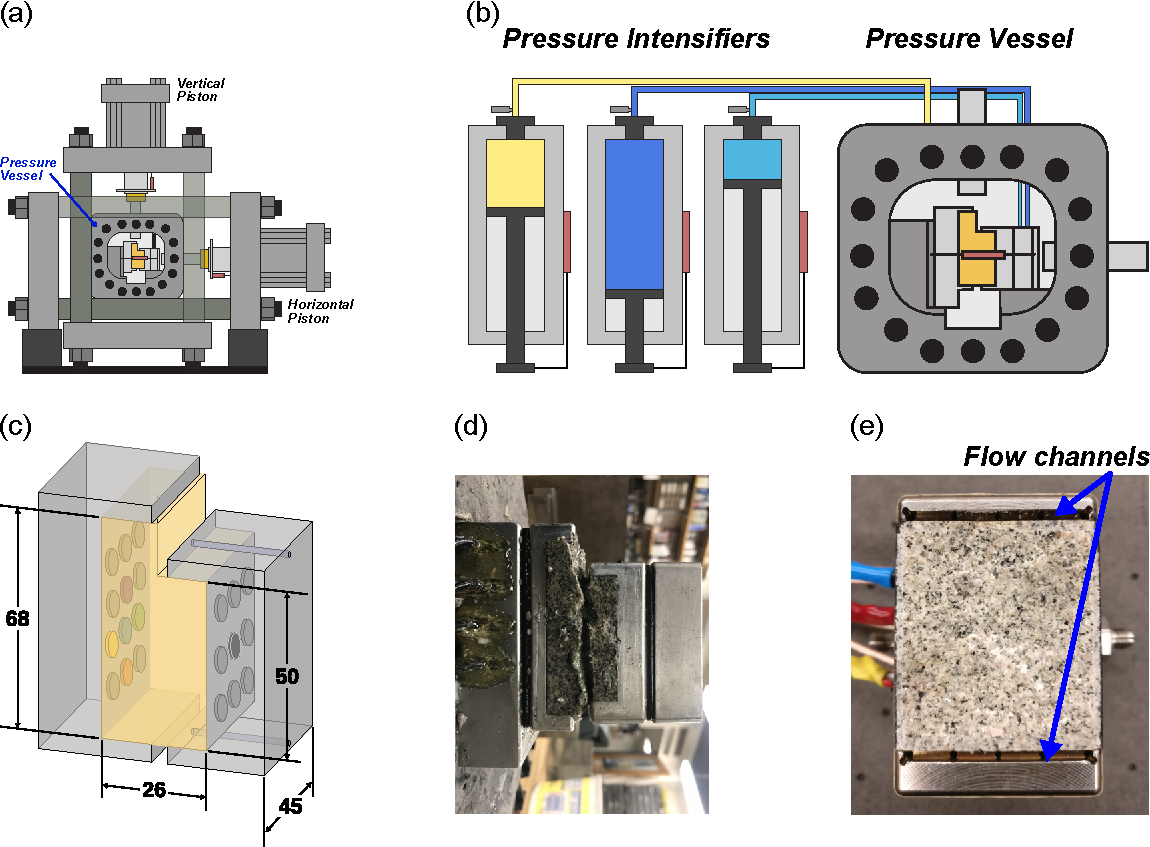
\includegraphics[width=0.9 \columnwidth]{experimental_configuration}
	\caption[]{(a) Experiments were conducted in the Penn State Rock and Sediment Mechanics laboratory using the Biaxial Deformation Apparatus (Biax). The Biax has servo-controlled vertical and horizontal pistons and a 10 kHz 24-bit analog to digital data recorder. (b) A pressure vessel is inserted into the Biax to create true triaxial loding. Pressure intensifiers control the confining pressure ($P_C$) and sample ($P_{PA}$ and $P_{PB}$ ) fluid pressures. (c) L-shaped samples of granite were loaded with platens containing piezoelectric transducers (p-polarized). The shorter platen has internal conduits to provide fluid at each end of the fracture plane via narrow channels (45 x 1 mm). Each channel is covered by a sintered porous fit (permeability $\sim 10^{-14}\ m^2$) and fed by five 1.6 mm diameter holes. The frits ensure homogeneous fluid distribution at each end of the fracture. After securing the sample in the loading platens it is sealed in a latex jacket to separate confining and pore fluids. (d) A photo of the sample after experimentation highlights the degree of roughness from in-situ fracture. (e) Post mortem photo showing the rough fracture and fluid flow channels. }
	\label{fig:samplesetup}
\end{figure*}

\newpage

\begin{figure*}[ht]
	\centering
	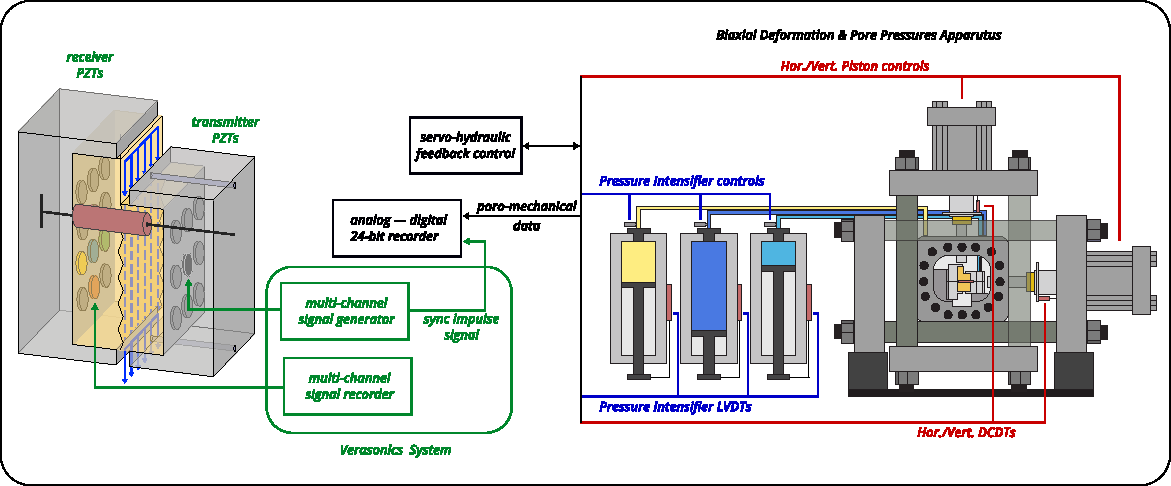
\includegraphics[width=0.9 \columnwidth]{exp_daq_v1}
	\caption[]{Schematic of the single direct shear configuration with the block diagram showing the main features of the data acquisition system for both the poro-mechanical and ultrasonic data. The Biax consists of two hydraulic pistons capable of applying vertical and horizontal loads in displacement or load control. Forces are measured using custom-built strain-gauge load cells mounted. The load cells have an amplified output of 5 V with an accuracy of 5 N and are calibrated with a Morehouse proving-ring. Displacements are measured with direct-current displacement transducers (DCDT), with an accuracy of $\pm 0.1 \mu m$. Each axis of loading is independently servo-controlled and all stresses, strains, fluid pressures and fluid volumes are recorded with ±10 V, 16-channel 24-bit analog-to-digital converters at 10 kHz and averaged to sampling rates of 100 Hz or 1 kHz. Fracture permeability was measured using upstream and downstream pore-pressure intensifiers. Active ultrasonic data were recorded using a Vantage TM Research Ultrasound (Verasonics) system. We use broadband (0.02-2 MHz) PZTs (APC International Ltd. 6.35 mm diameter compressional crystals), which were successively pulsed every 1 ms on the transmitting side and the recording rate at the receiver side was 25 MHz. The input signal is a half sine with a frequency of 500 kHz. Also, a pulse from the Verasonics system accompanied the PZT excitation and is recorded by the 24-bit analog-to-digital data acquisition system. This allows us to sync the ultrasonic to poro-mechanical data and then analyzed to measure changes in the permeability and elasticity of the fractured rock samples, explained more fully in the signal analysis procedure.}
	\label{fig:data_aq}
\end{figure*}

\newpage


\subsection{Experimental Procedure}
\paragraph{}
Each experiment commenced with extensive sample preparation in which the Westerly granite was cut and notched, sealed in a latex jacket, and then placed inside the pressure vessel. After sealing the pressure vessel and loading the sample, inlet and outlet flow were pressurized to 4 MPa and 2 MPa, respectively. At this stage there was no flow because Westerly granite matrix permeability is very low ($< 10^{-20}\ m^2$ ) and the confining fluid pressure (around the jacketed sample) is much larger than the pore pressure, preventing flow of water around the sample.
A shear load was then applied with the vertical piston in displacement mode at a constant rate of 10 $\mu m/s$. Samples fractured in-situ after reaching a critical stress of $ \approx $55 MPa, after which we locked the vertical piston. Fluid flow and acoustic emissions were measured during fracture, but here we focus on dynamic stressing which was implemented via oscillations of the effective normal stress.
\paragraph{}
Oscillations of applied normal stress were implemented with the horizontal loading piston at prescribed amplitudes (0.2 to 3 MPa) and frequencies (0.1, 1, 10, 40 Hz). Pore pressure oscillations were achieved by oscillating $P_{PA}$ while holding $P_{PB}$ constant at amplitudes of 0.2 to 3 MPa and frequencies of 0.1, 1, 10 Hz. Multiple sets of normal stress and pore pressure oscillations of varying amplitudes and frequencies were applied to investigate: (1) repeatability and direct comparison between the two modulated stresses (normal stress and pore pressure) and (2) amplitude and frequency dependencies of the measured response. Post-fracture dynamic stressing is plotted in Figure \ref{fig:exp_seq}d (highlighted in yellow) and shows the normal stress (red) and pore pressure (blue) oscillations.
To investigate the effect of shearing and resulting changes in fracture aperture and generated wear material on elastic nonlinearity and permeability, the sample was sheared in two 4 mm, (held at $ \sigma_{NS} $ = 20 MPa) stages. After each shearing stage the oscillation protocol was applied to the sample. Initially,the in-situ fracture was quite rough with fines throughout, but the effect of shear reduces and changes this roughness; the old contacts were broken and new contacts formed, changing the extent to which the two halves of the fracture were mated. Throughout shear the size, shape, and amount of wear material, or fines, continuously evolves and likely has complicated effect on fluid flow. This allows for investigation of how fracture aperture is related to the elastodyamic and hydromechanical properties.

\newpage


\begin{figure*}[ht]
	\centering
	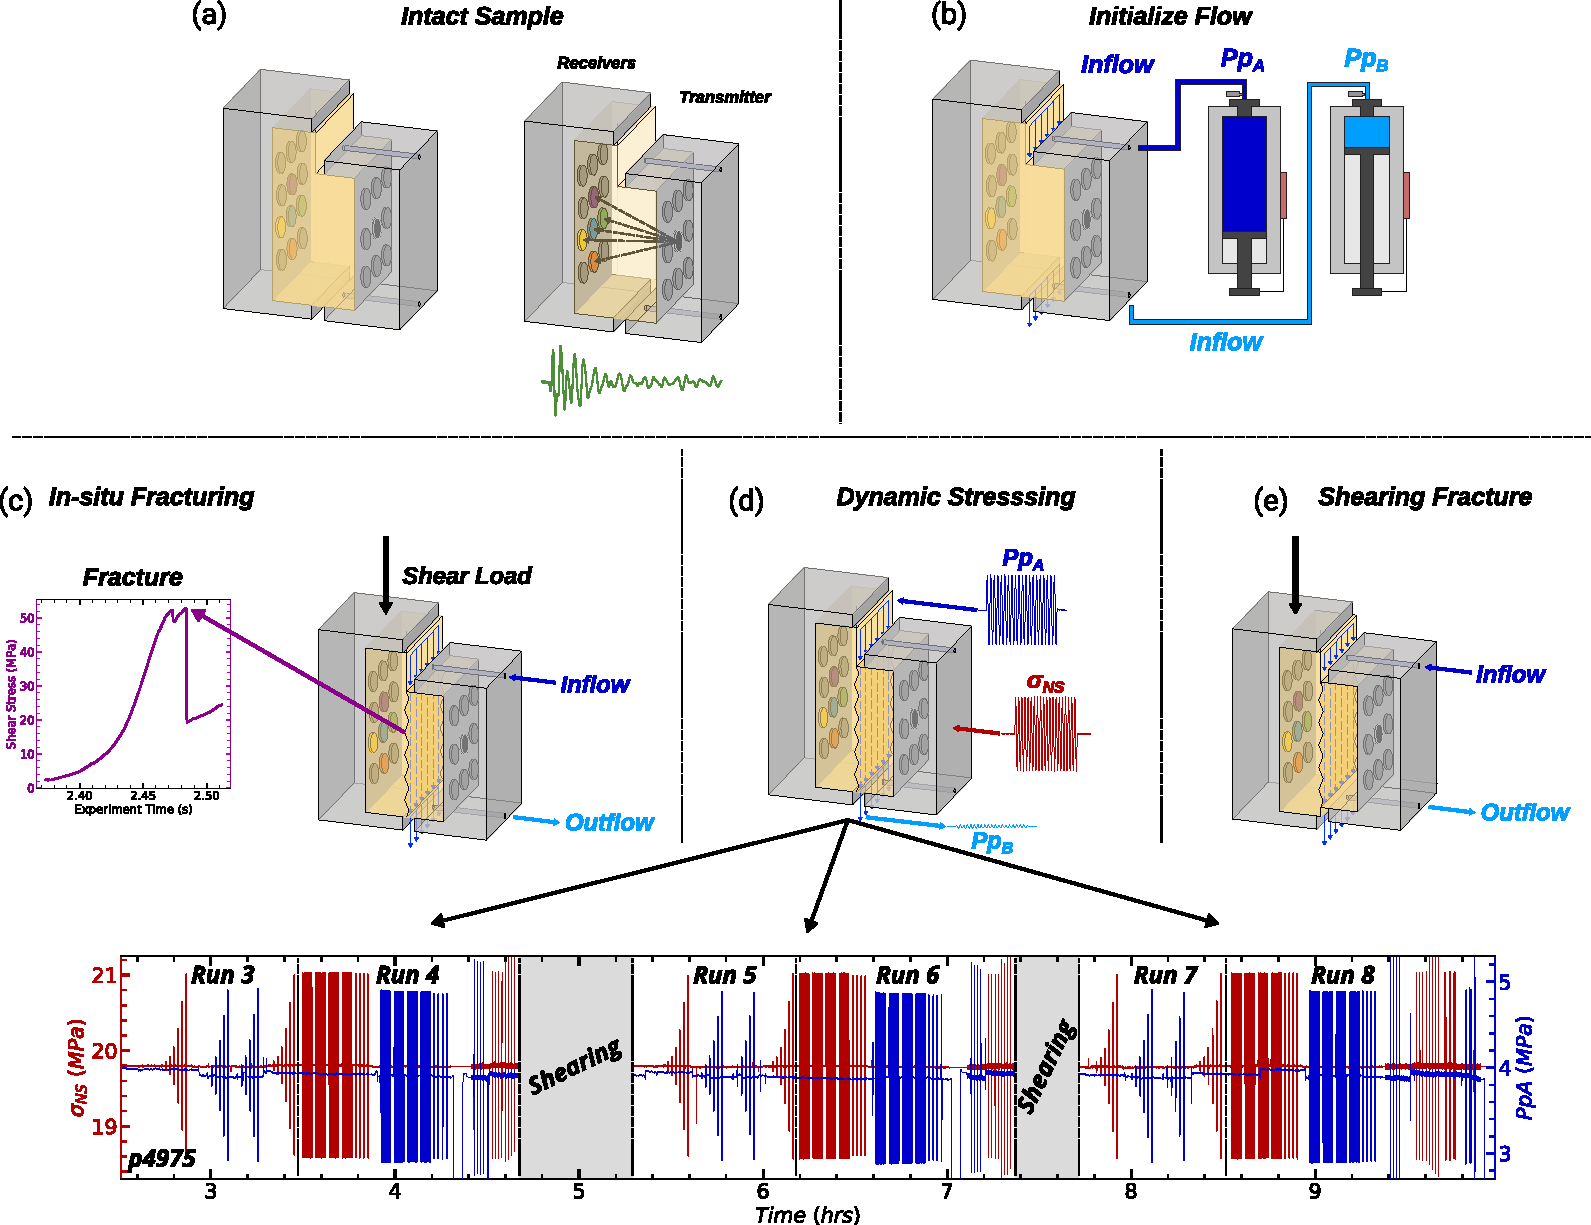
\includegraphics[width=0.99\columnwidth]{exp_sequence_v3}
	\caption[]{(a) Sketch showing sample dimensions and approximate PZT transmitter - receiver ray paths.
		(b) Fluid flow and pore pressure with inlet ($P_{PA}$ = 4 MPa) and outlet ($P_{PB}$ = 2 MPa).
		(c) Shear stress on the fracture plane was increased by advancing the long end of the L-shaped sample at a constant rate of 10 $\mu m/s$ while holding the short end in place. Fracture occured in two stages at $ \approx $55 MPa.
		(d) Sketch showing the oscillation protocol applied to the freshly fractured sample. Multiple sets of $P_{P}$ and $ \sigma_{NS} $ oscillations of varying amplitude (up to about $ \pm $ 1 MPa) and frequency (0.1, 1, 10 and 40 Hz) were applied.
		(e) Fractures were sheared in two stages, each followed by the dynamic stressing protocol.}
	\label{fig:exp_seq}
\end{figure*}


\newpage

% \subsection{Dynamic Perturbations of the Fracture Normal Stress}
% The fractured samples were dynamically perturbed via pore pressure ($P_P$) and normal stress ($\sigma_{n}$) oscillations. Following the procedure described by Candela et al., 2015, pore pressure oscillations were achieved by oscillating $P_{PA}$ while holding $P_{PB}$ constant. Conversely, normal stress oscillations were applied by oscillating the horizontal piston of the load frame at prescribed amplitude and frequency.
% As depicted in Figure 2a, multiple sets of Pp and $\sigma_n$ oscillations of varying amplitude (up to about $\pm$ MPa) and frequency (0.1, 1, 10 and 40 Hz) were applied to investigate the repeatability as well as amplitude and frequency dependencies of the measured response. Similar parameters were used for $P_P$ and $\sigma_{n}$ oscillation sets in order to apply similar effective stress perturbations and allow making comparisons between $P_P$ and $\sigma_{n}$ stimulations.


\subsection{Permeability Measurements}
\paragraph{} We measured flow rates independently at the fracture inlet ($Q_A$) and outlet ($Q_B$) using the outputs of LVDTs on the pressure intensifiers. After verifying the steady state flow condition ($Q_{A} - Q_{B}  \leq 5 \% $), Darcy’s law was
used to calculate permeability k:
\begin{equation} \label{eq:perm}
	k = \frac{\mu L}{S} \frac{Q}{\Delta P_P}
\end{equation}
where $Q = \frac{1}{2} (Q_A + Q_B )$ is the average flow rate ($\frac{m^3}{s}$), $\mu$ is the fluid viscosity ($10^{-3} Pa\cdot s$) at 20\textdegree\ C, $L$ is the flow path given by the length of the sample (50 mm) and $S$ is the cross section perpendicular to the flow path (45 x 26 $mm^2$).
\paragraph{} Specifically, k is the bulk permeability, that is, the permeability of the surrounding rock matrix (on order of $10^{-21} m^2$) and of the fracture. Alternative calculations of permeability are valid [Zhang et al., 2017; Ishibashi et al., 2018], however we are interested in relative changes in permeability in response to dynamic stressing, rather than the absolute value of fracture permeability.


\subsection{Ultrasonic Measurements: Active Source}
Ultrasonic waves transmitted through the fracture were recorded continuously in each experiment. Half-cycle sinusoidal pulses with an amplitude of 40 V and center frequency of 500 kHz were emitted consecutively from each transmitting transducer (9 piezoelectric discs arranged in a 3 x 3 matrix embedded within the right-hand loading platen in Figure 1b) with a pulse repetition frequency of 100 Hz or 1000 Hz during the low and high frequency ($\geq 10$ Hz) stress oscillations, respectively. The waveforms were amplified ($\sim 40$ dB) and recorded for all the receiving transducers (12 piezoelectric discs arranged in a 4 x 3 matrix embedded within the left-hand loading platen in Figure 1b). In this study we utilized 1 transmitter and 3 receivers. 

\newpage

\begin{figure*}[ht]
	\centering
	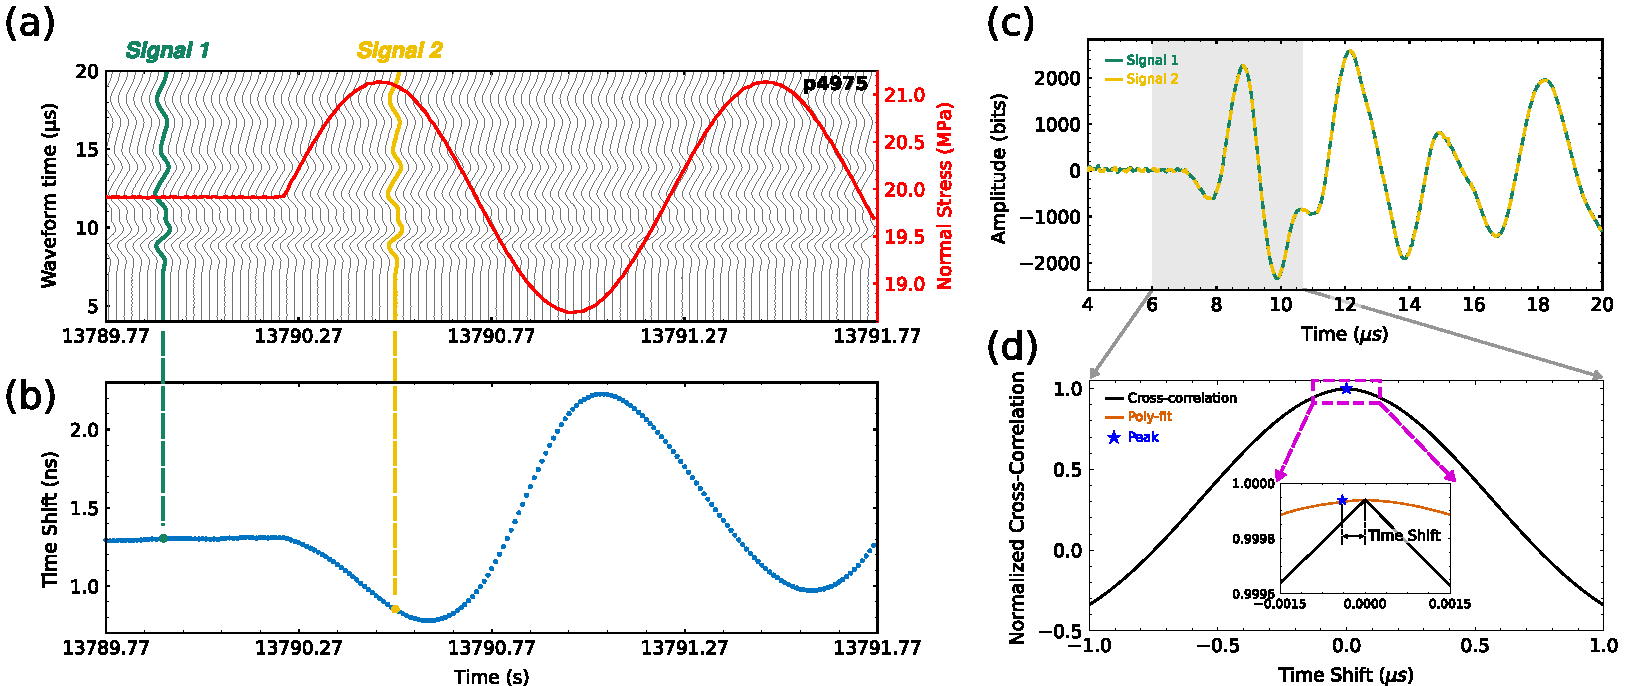
\includegraphics[width=0.9 \columnwidth]{xcor_fig_v3}
	\caption[]{(a) Excerpt from Run 4 of experiment p4966 (see Fig. 3 for context in p4975) shows part of a 1 Hz, 1 MPa normal stress oscillation (red) and the concurrent raw ultrasonic waveforms (grey). The number of waveforms in the waterfall plot has been decimated for clarity. (b) Time shift was calculated by cross-correlating the waveforms with a reference waveform. (c) An example of a reference, unperturbed, waveform (green) and perturbed waveform (dashed yellow) highlights
		the similarity. (d) The maximum linear correlation between the reference and perturbed waveforms from cross-correlation is used to determine the time shift. The inset shows improvement of time shift calculations with a 2nd order polynomial fitting procedure.}
	\label{fig:xcor_poly}
\end{figure*}

\newpage



%--------------------------------------------------------------------------
%RESULTS
%--------------------------------------------------------------------------

\section{Results}
\paragraph{}
We combine ultrasonic data, strain measurements, and permeability to document the nonlinear elastodynamic response and poromechanical effects of dynamic stressing. Here, we draw from an extensive set (>10) of experiments, calibrations, and tests to focus on data from two distinct experiments with a range of stressing amplitudes and frequencies.

\subsection{Nonlinear elastodynamic and hydraulic responses}
\paragraph{}
Linear elasticity does not adequately describe the behaviour of rocks. Even undamaged rocks exhibit a range of nonlinearity due to a variety of structural features such as microcracks and soft grain boundaries (Rivière et al., 2015). When fractured or damaged, rock's nonlinearity is further affected by contact acoustic nonlinearity at fracture interfaces. The characteristic responses to dynamic stressing (transient softening, velocity modulation, and slow recovery) as shown in Figure \ref{fig:delc_delk_calc}, are indicative of nonlinear mesoscopic elasticity (Guyer and Johnson, 2009) and highly informative on rock microstructure, fractures, and intergrain contacts. Interestingly, these are the features that also control the hydraulic properties of rock.

\paragraph{}
Through our active source ultrasonic monitoring we characterize the elastodynamic properties of the fractured Westerly granite by quantifying its response to dynamic stressing. Figure \ref{fig:delc_delk_calc} demonstrates typical recorded elastodynamic and hydraulic responses to a 1 Hz, 1 MPa normal stress oscillation in experiment p4966. We characterize the elastodynamic response with three parameters to describe the nonlinearity, $ \Delta c/c_0 $, $ dc/c_0 $, and $ \Delta A/A_0 $. We observe steady-state wave velocity $ c_0 $ before dynamic stressing which causes an immediate reduction followed by a further transient decrease. Wave velocity recovers to a new steady-state value that we quantify as  $ \Delta c $.
The RMS wave amplitude is calculated in the time domain of a window comprising the first arrived p-wave, related to fracture stiffness. Dynamic stress oscillations result in a sudden decrease in amplitude relative to the initial value  $ A_0 $ to a new temporary non-equilibrium state. Therefore, both $ \Delta c/c_0 $ and $ \Delta A/A_0 $ quantities are nonlinear parameters that demonstrate the transient effect of dynamic loading on fracture stiffness, for a range of stress amplitudes and frequencies. Though RMS amplitude can be extracted from our data, it is not the main focus of this paper, but some results are reported in Supplemental Materials.  
Another nonlinearity parameter that we identify is modulation of the wave velocity, $ dc $, during oscillations at frequencies that are harmonics of the driving frequency. This quantity represents the average amplitude of wave velocity modulations during dynamic perturbations after the system reaches a non-equilibrium steady-state. Finally, after being stressed, the fractured rock exhibits long-term ``recovery'' trending toward the initial $ c_0 $ value, in which the wave velocity or amplitude evolves to a new steady state. The wave velocity evolution from post-oscillation to initial $ c_0 $ is well described by a logarithmic function of the form $ c = p_1\ \log{t} + p_2 $, where $p_1$ is the slope (recovery rate) $ \dot c $ and $p_2$ is the intercept. 

\paragraph{}
We also measure the evolution of permeability due to dynamic stressing and correlate it with nonlinear elasticity. In our experiments elastic waves propagate orthogonal to the fracture plane and their amplitude, phase and speed depend on the fracture aperture. Hydraulic measurements, comparing inlet and outlet fluid flow across the fracture plane, tell a similar story; permeability and transmissivity reveal changes in fracture aperture.
The stress-induced changes in permeability are captured by two parameters: (1) The transient change in permeability $ \Delta k/k_0 $ defined as the \%-change due to the imposed normal stress or pore pressure oscillations, normalized by the pre-oscillation permeability $ k_0 $ as illustrated in Figure \ref{fig:delc_delk_calc}c [Candela et al., 2014] and (2) the logarithmic rate of permeability recovery after the transient increase $ \dot k $ where $ k = q_1\ \log{t} + q_2 $, where $q_1$ is the slope (recovery rate) and $q_2$ is the intercept.
Figure \ref{fig:delc_delk_calc} shows the pre-oscillation permeability $ k_0 $ and the post-oscillation permeability $ k = k_0 + \Delta k $ calculated by averaging the measured values over 10- and 1-s time windows. Calculation discontinuities in permeability measurements shown in Figure \ref{fig:perm_calc} correspond to times for which inlet/outlet flow rate difference exceeds the 5\% threshold that we impose to ensure steady state flow. Permeability during dynamic stressing is indeterminate because there is no steady-state flow and the diffusion time across the fracture is slower than the higher oscillation frequencies (10 and  40 Hz). 

\paragraph{}
To better illustrate how the elastodynamic and hydraulic properties of fractured rock change in response to dynamic perturbation we show an excerpt from the post-fracture stage of experiment p4975 in Figure \ref{fig:NS_p4975_run3b_01Hz}.
Figure  \ref{fig:NS_p4975_run3b_01Hz} demonstrates how the inlet and outlet flow rates evolve during a 0.1 Hz normal stress oscillation; three colorbars highlight zoomed cycles in Figure \ref{fig:bowties}. Note the clear evidence of compression and tension in the fracture normal displacement with increased and decreased normal stress (Figure 7). The inlet $ Q_A $ flow rate is in phase with the imposed stressing, but the outlet flow $ Q_B $ is 180$\degree$ out of phase and of a much smaller magnitude than that of the inlet;  furthermore, the amplitude trends are modulated throughout the oscillation. For sufficiently long duration stressing the wave velocity modulations reach a steady-state. These observations demonstrate the magnitude of changes we are characterizing and also reinforce that the fracture is continuously evolving during the dynamic perturbations; contacts undergo compression and tension resulting in changing fluid flow paths along the fracture.

%This figure also includes hysteresis plots that show how the wave velocity vary as a function of stress. Throughout this long oscillation the velocity-flow hysteresis loop generally evolves to a lower velocity and lower flow rate and the loop becomes slightly more closed. We also observe this general decrease in wave velocity as a function of applied stress throughout the history of the oscillation.If the oscillation persists long enough, the wave velocity modulations reach a steady-state. These observations demonstrate the magnitude of changes we are characterizing and also reinforce that the fracture is continuously evolving during the dynamic perturbations; contacts undergo compression and tension resulting in changing flow paths across the fracture.

\paragraph{}
In subsequent subsections we discuss how nonlinear elastodynamic and hydraulic parameters $\Delta c/c_0$, $ \Delta k/k_0 $, $dc/c_0$, and $\Delta A/A_0$ vary with normal stress and pore pressure oscillation amplitudes and frequencies. We also discuss how these results are affected by shearing for both experiments p4966 and p4975.

\newpage

\begin{figure*}[ht]
	\centering
	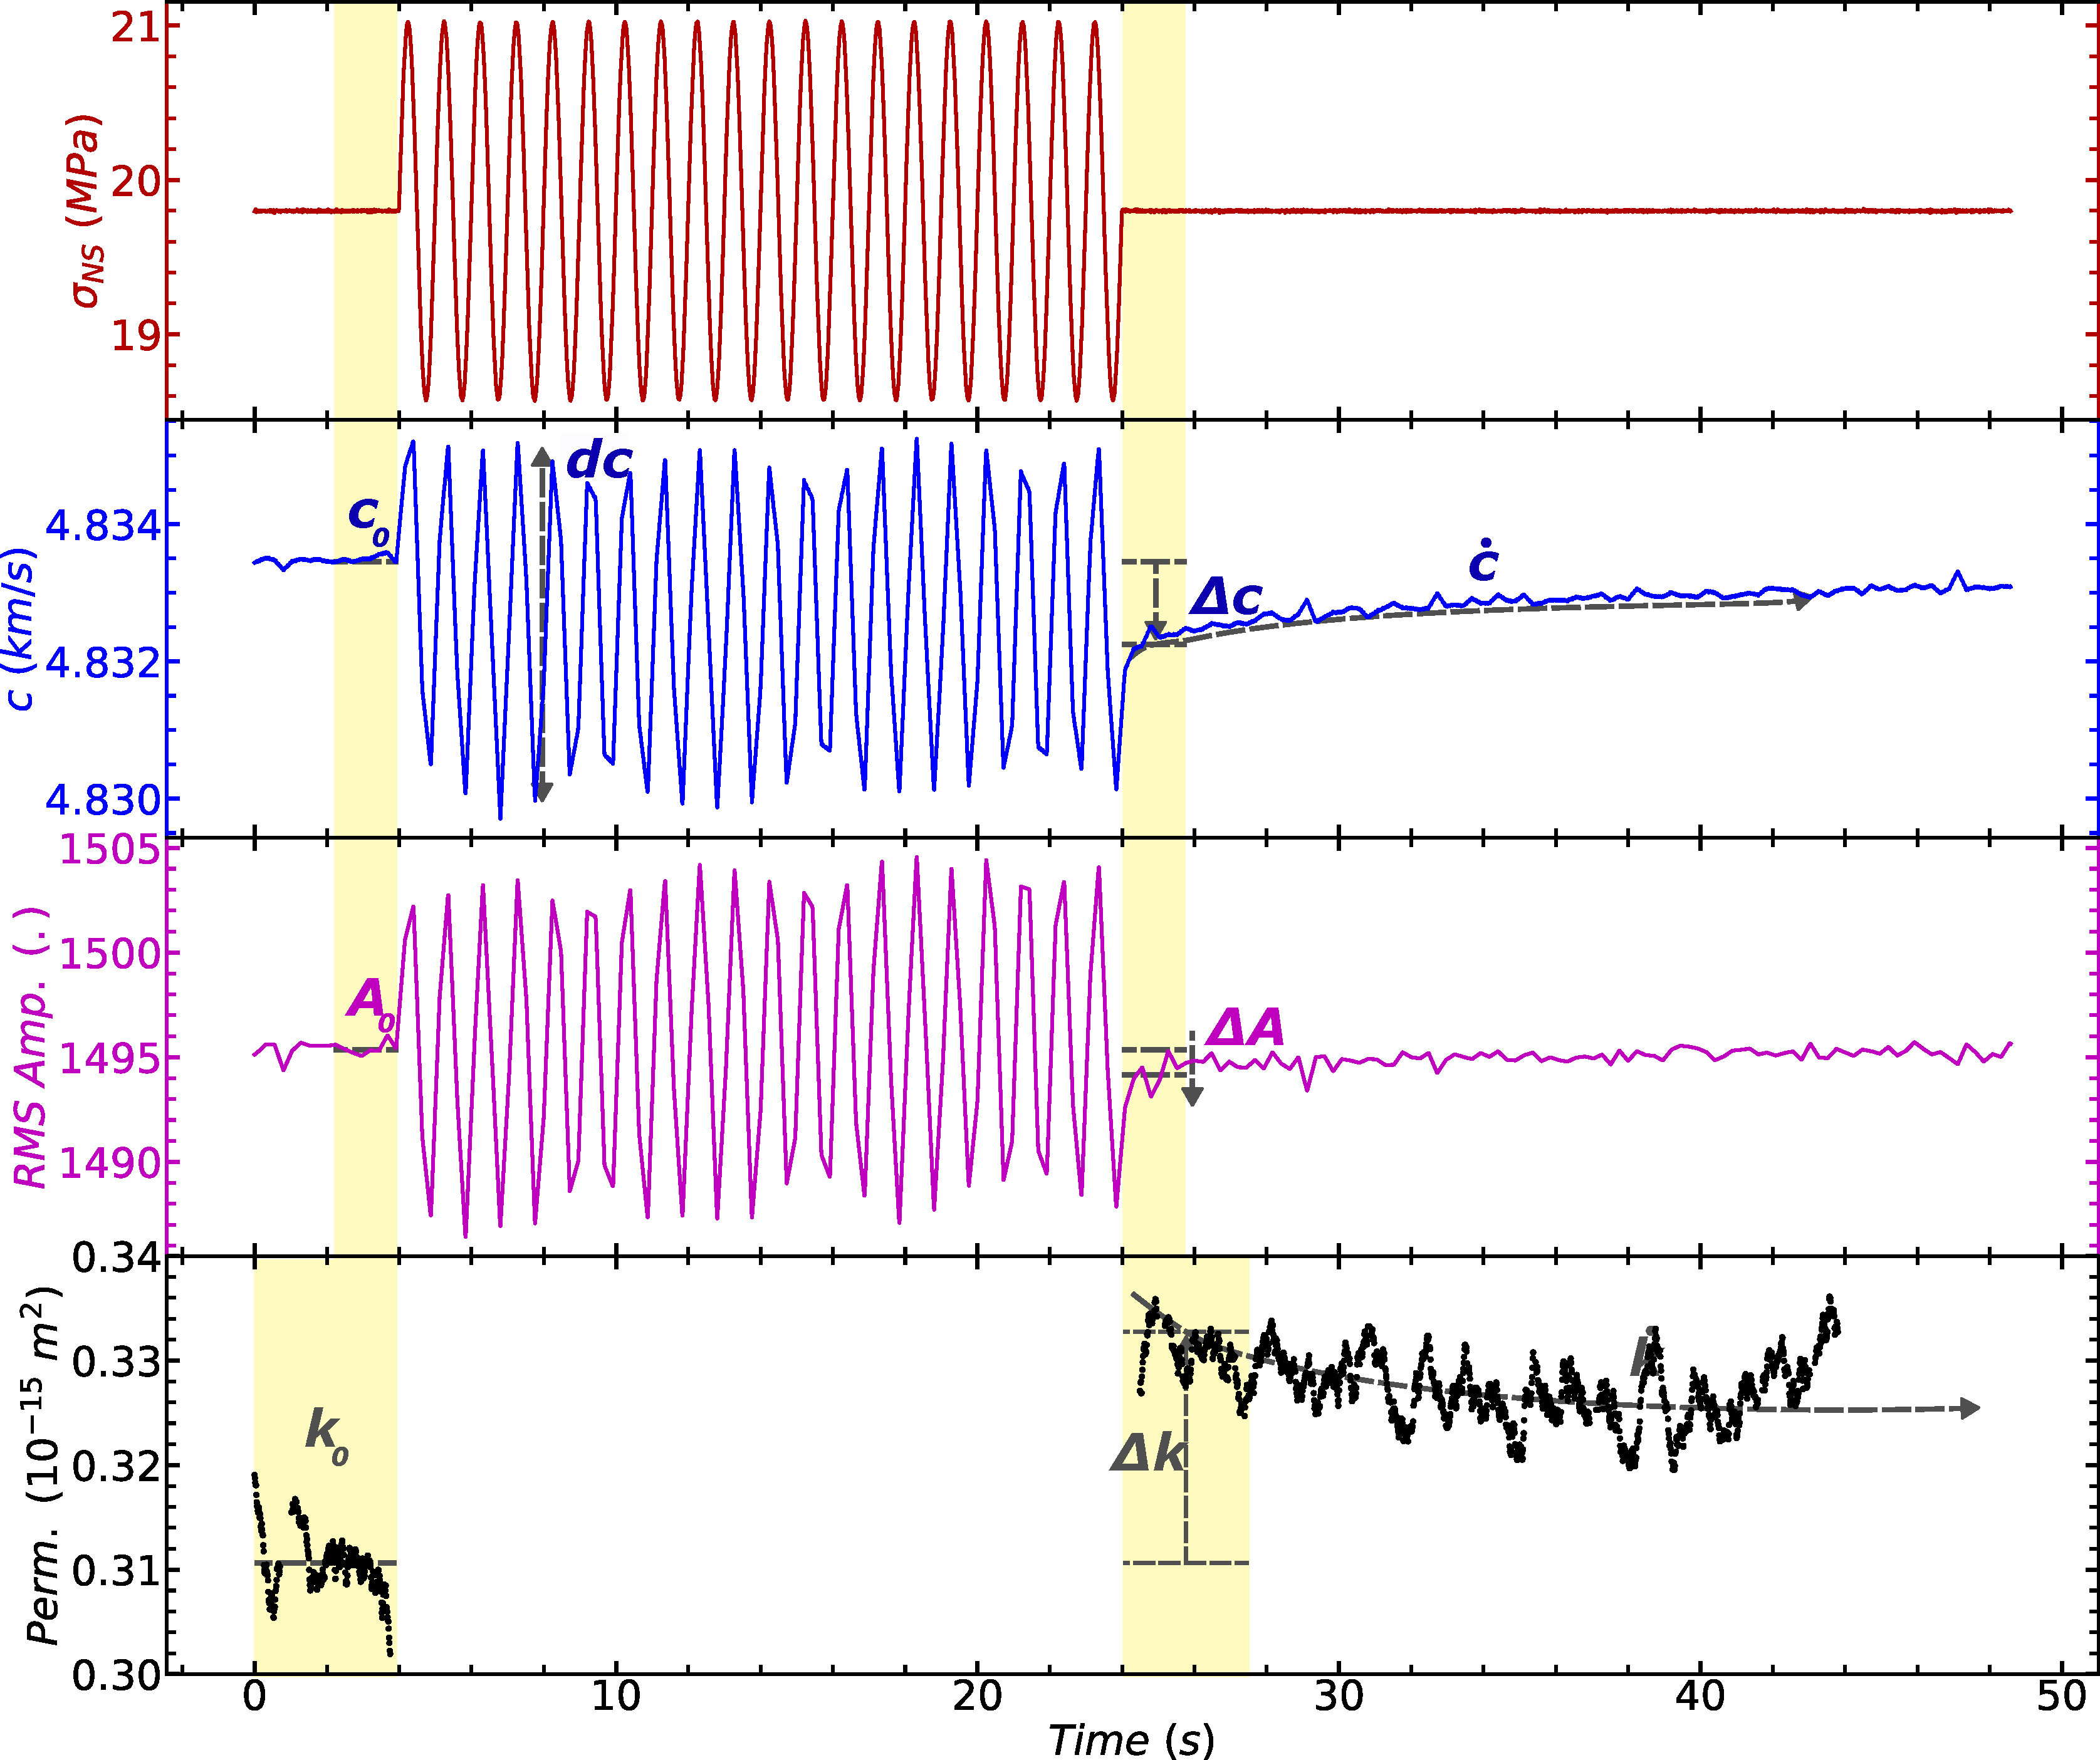
\includegraphics[width=0.9\columnwidth]{NsVelRmsPerm_v2_edit}
	\caption[]{Details of elastodynamic and hydraulic response to dynamic stress oscillation, see Run 4 of p4975 in Fig. 3. Wave velocity and permeability changes are calculated using the measured values before and after oscillations averaged over the time windows indicated by yellow boxes. Permeability measurements are shown only for steady state flow when the inlet/outlet flow rates differ by $ < 5 \% $. We measure the dynamically induced changes in p-wave velocity ($ \dot c$) and permeability ($\dot k$) as well as their changes $\Delta c$ and $\Delta A$ relative to the initial values $c_0$ and $A_0$. Furthermore, we measure the average change in p-wave velocity during dynamic stressing oscillations as $ dc $.}
	\label{fig:delc_delk_calc}
\end{figure*}

\newpage

\begin{figure*}[ht]
	\centering
	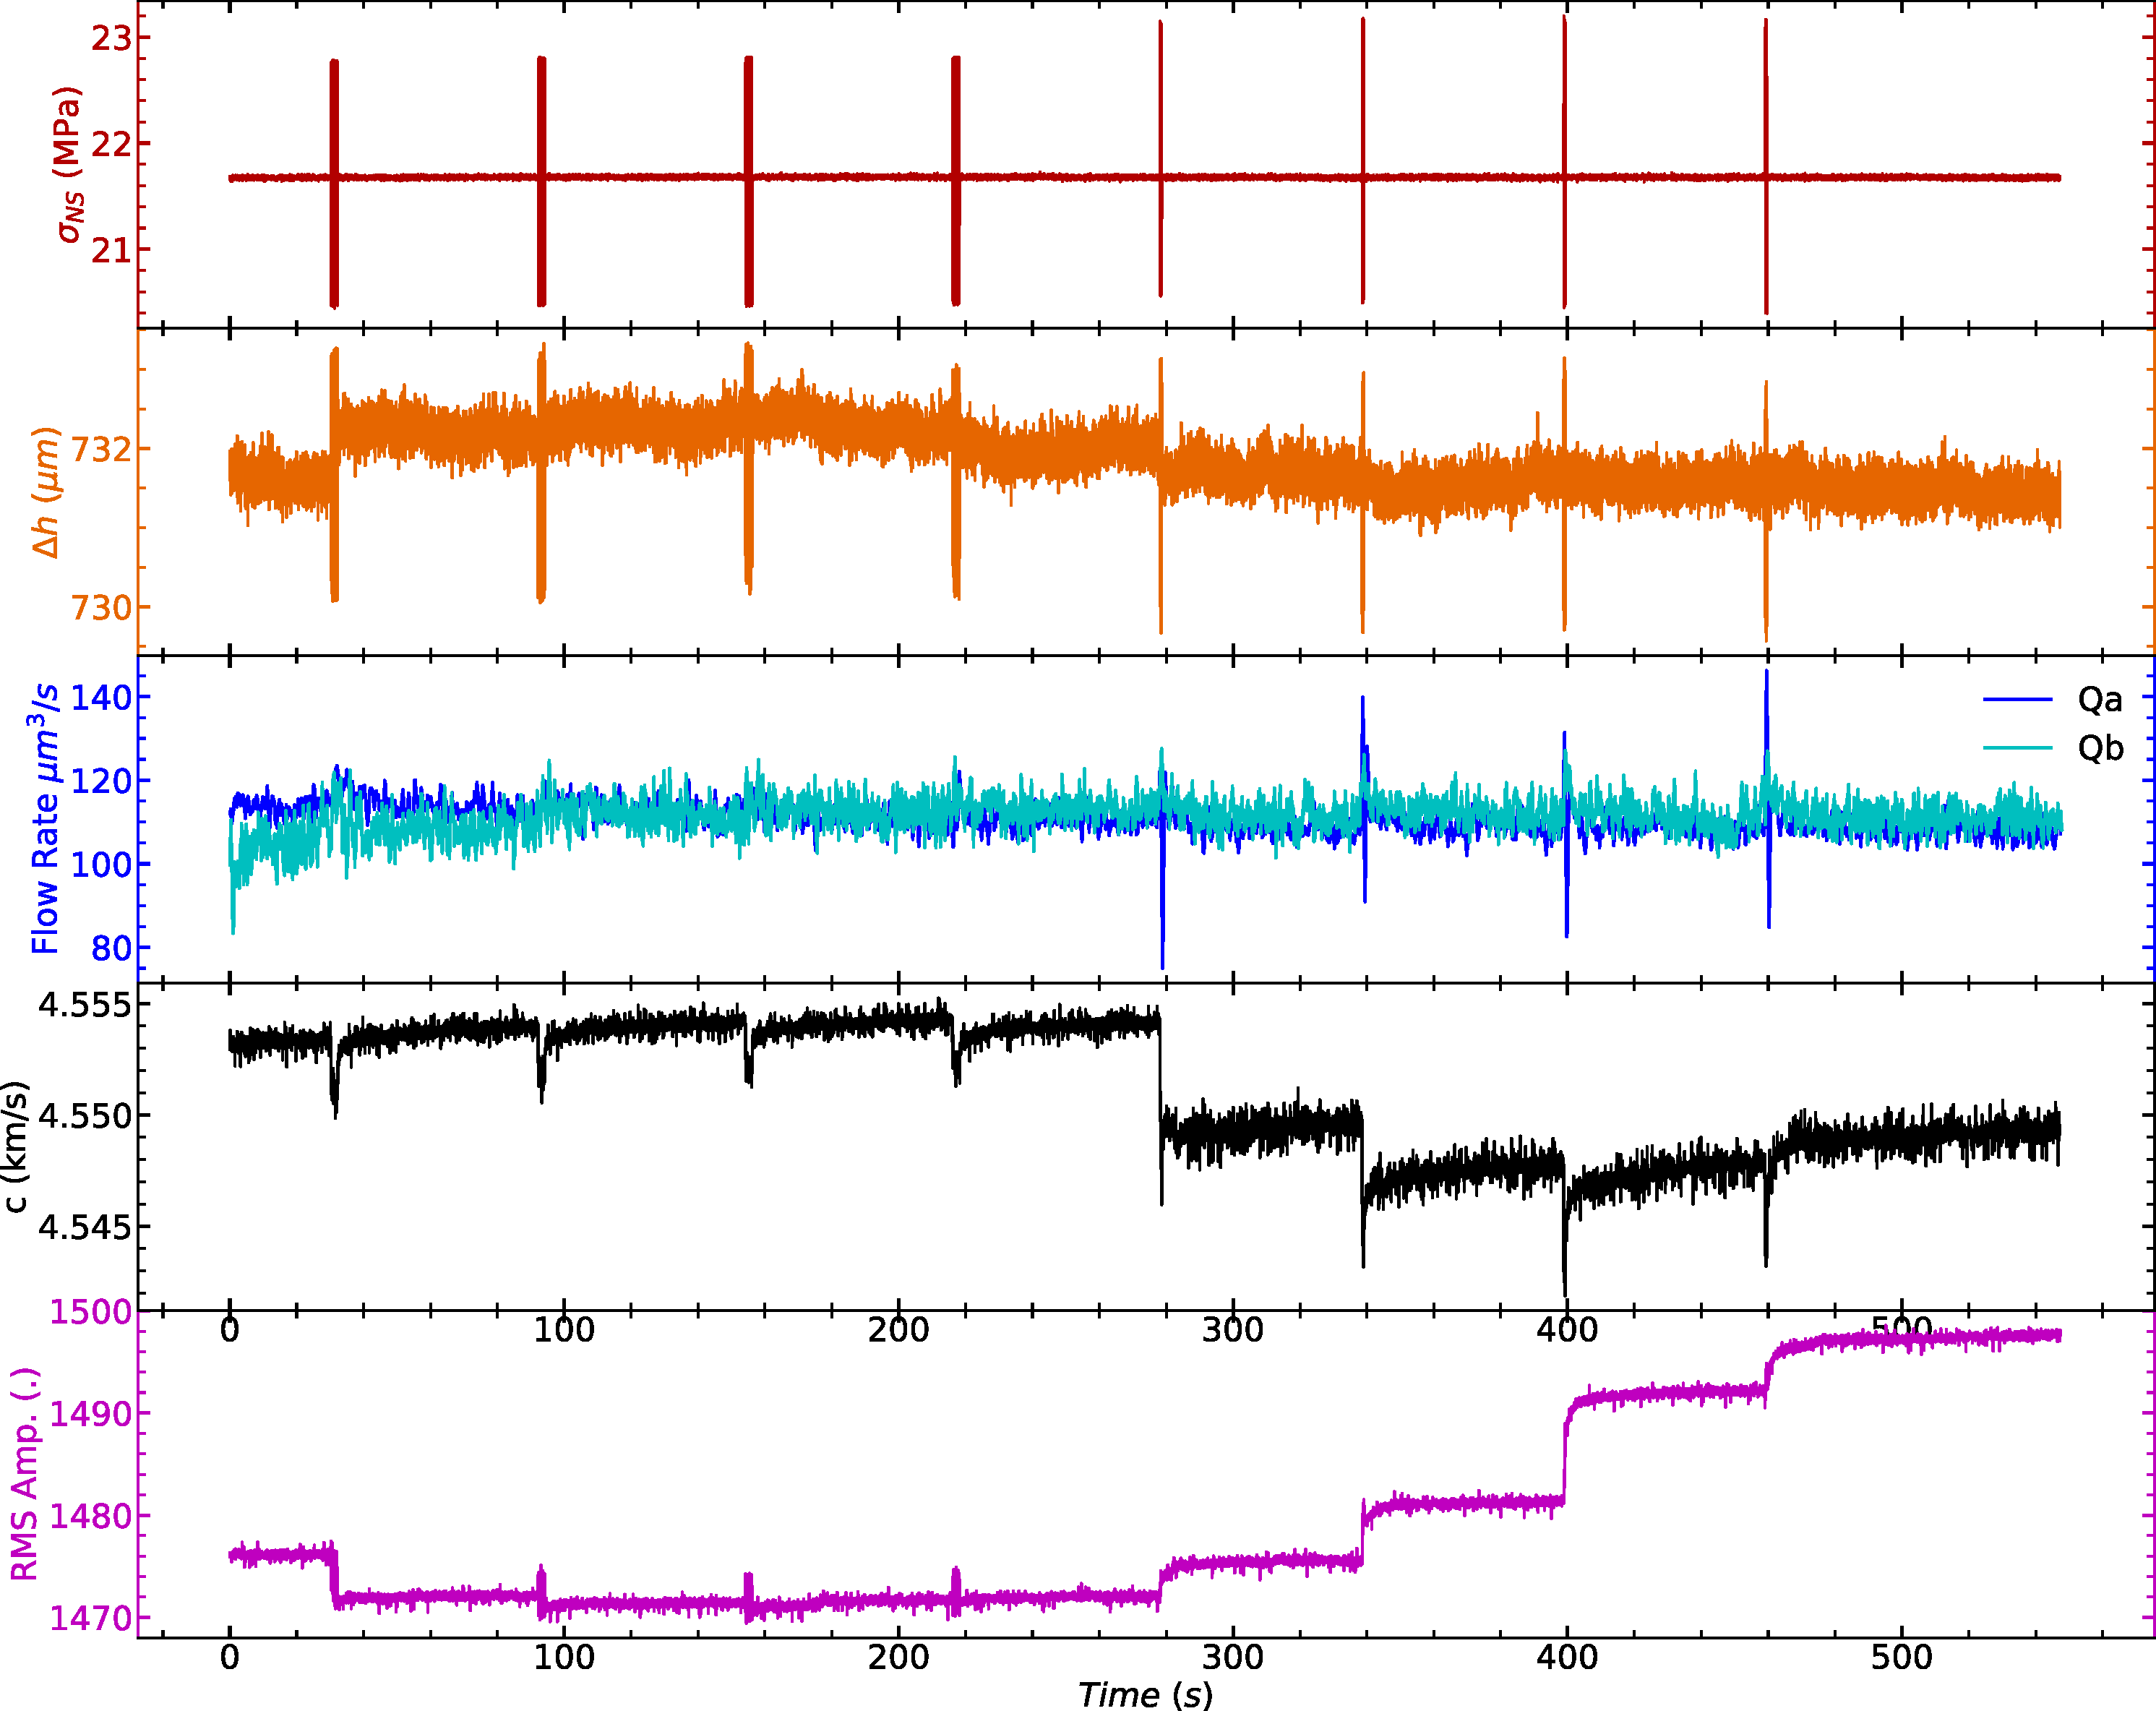
\includegraphics[width=1\columnwidth]{NS_p4975_run4}
	\caption{Elastodynamic and hydraulic data for one full dynamic stressing protocol with pore pressure oscillation (See Fig. 3: Run 4 experiment p4975. These data are for center transmitter to blue receiver in Figure 2. Two sets of 1-MPa amplitud pore fluid pressure oscillations were imposed at frequencies of 0.1, 1, 10 and 40 Hz. In all cases p-wave velocity shows a transient reduction upon dynamic stressing followed by recovery. Oscillations begin with a pore pressure increase and thus fracture aperture $\Delta h$ increases initially, as effective stress drops, and then undergoes a transient change that varies with stressing history. Wave amplitude also shows a complex response to stress oscillations including both transient and long term changes. }
	\label{fig:run4_p4975}
\end{figure*}

\newpage

\begin{figure*}[ht]
	\centering
	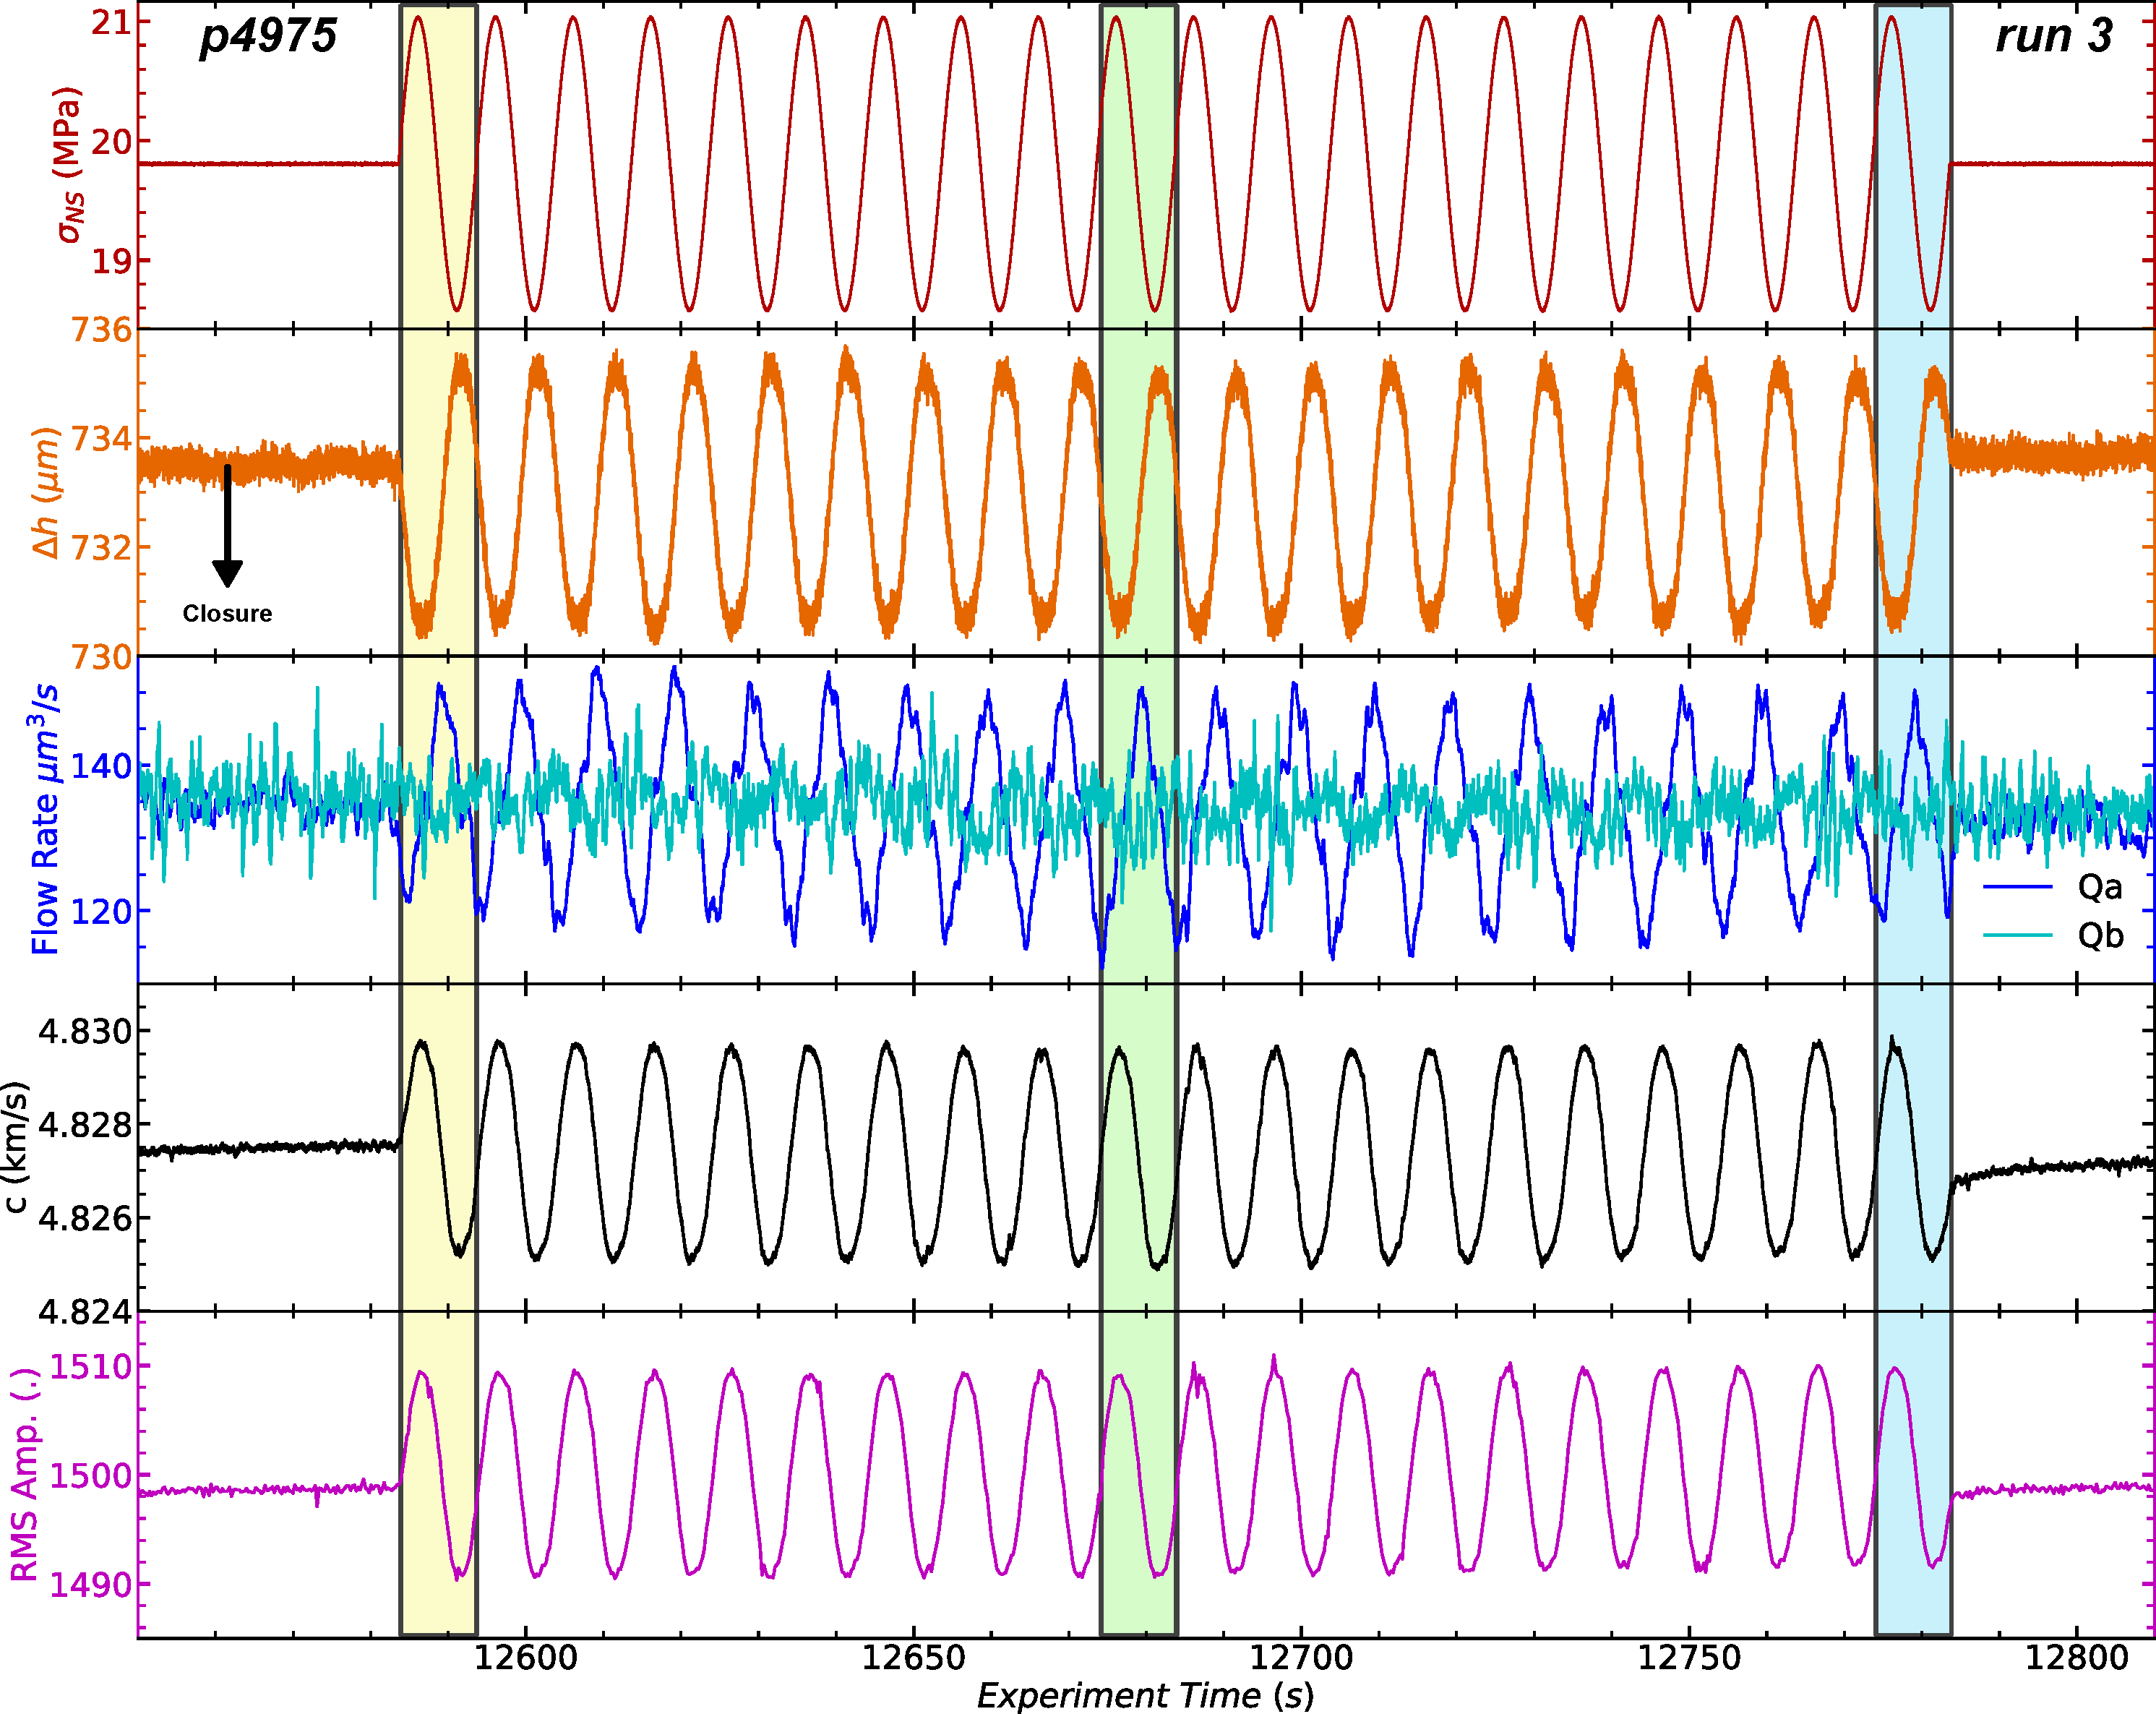
\includegraphics[width=0.9\columnwidth]{NS_p4975_run3}
	\caption[]{Elastodynamic and hydraulic data for one set of applied normal stress oscillations frequency of 0.1 Hz and amplitude of 1 MPa (See Fig. 3). Fracture aperture decreases initially as normal stress increase and then varies in phase with fracture normal stress. Fluid flow data from the fracture inlet (PpA) and outlet (PpB) document the transient response to changes in fracture aperture and stress state. Note that inflow is phase lagged relative to fracture aperture. Elastic wave speed and amplitude are shown for the direct path pair (center transmitter to blue receiver in Figure 2). Three sections are highlighted showing one full cycle in the beginning, middle, and end of the normal stress oscillation. }
	\label{fig:NS_p4975_run3b_01Hz}
\end{figure*}

\clearpage


\subsection{Dynamic Stress-induced Changes in Permeability and Wave Velocity}
\paragraph{}
One hypothesis driving our work is that transient elastic softening and nonlinear elasticity can provide information about rock fracture properties via dynamic stressing. A corollary is that changes in fracture aperture cause both changes in permeability and elasticity. A more complete understanding of both physical phenomena is important for understanding processes that control energy production and waste storage. In this section, we report and compare the stress amplitude and frequency dependencies for both sets of parameters. 

The dependency of $ \Delta k/k_0 $ on the amplitude of normal stress and pore pressure oscillations is shown in Figure \ref{fig:perm_ns_amp}, which additionally differentiates the order in which the 1 Hz oscillations sets were imposed. We observe in experiments p4966 and p4975 fairly similar $ \Delta k/k_0 $ results for the post-fracture case. This is not entirely surprising because, though these experiments pertain to different samples/fractures, both samples are Westerly granite and the same loading conditions were used to produce approximately planar fractures resulting in presumably similar apertures and amount of fragmentation. Interestingly, this similarity deteriorates especially for pore pressure oscillations after the first shear phase of the experiments. After shearing the fractures (5 mm in p4966 and 4 mm in p4975) fragmented wear material develops in the interface, which inevitably complicated flow -- clogging and unclogging during the pore pressure oscillations such that wear material was dislodged from certain parts of the fracture or lodged in other parts.

Compared to dynamic stressing via pore pressure, permeability $ \Delta k/k_0 $ is relatively unaffected by oscillations of the applied normal stress oscillations for post-shear cases. This suggests that gouge material generated during shear is not mobilized to the degree it is by pore pressure, perhaps because pore fluids are more effective in moving gouge material and clogging/unclogging flow paths. This mechanism is not fully understood but likely plays a significant role in this complicated process.

We observe that the relative permeability change $ \Delta k/k_0 $ generally scales with the amplitude of 1 Hz normal stress post fracture and pore pressure oscillations and that the order in which oscillations were applied have an effect on the permeability enhancement. There are cases especially for post-shear oscillations where small oscillation amplitudes ($< $ 0.5MPa) result in a modest reduction in permeability for normal stress oscillations, but can result in relatively larger reductions for Pore pressure oscillations. Despite scatter, fairly similar relationships are observed for the two separate experiments.

Order of oscillations does not necessarily correlate to a specific permeability enhancement or reduction, but does have an effect on the overall results. This is most likely due to the fact that the pore pressure and normal stress oscillations do not strictly alternate, although the order is consistent in post-fracture, post-shear 1, and post-shear 2 parts of the experiments as shown in (reference your protocol).



\clearpage

\begin{figure*}[ht]
	\centering
	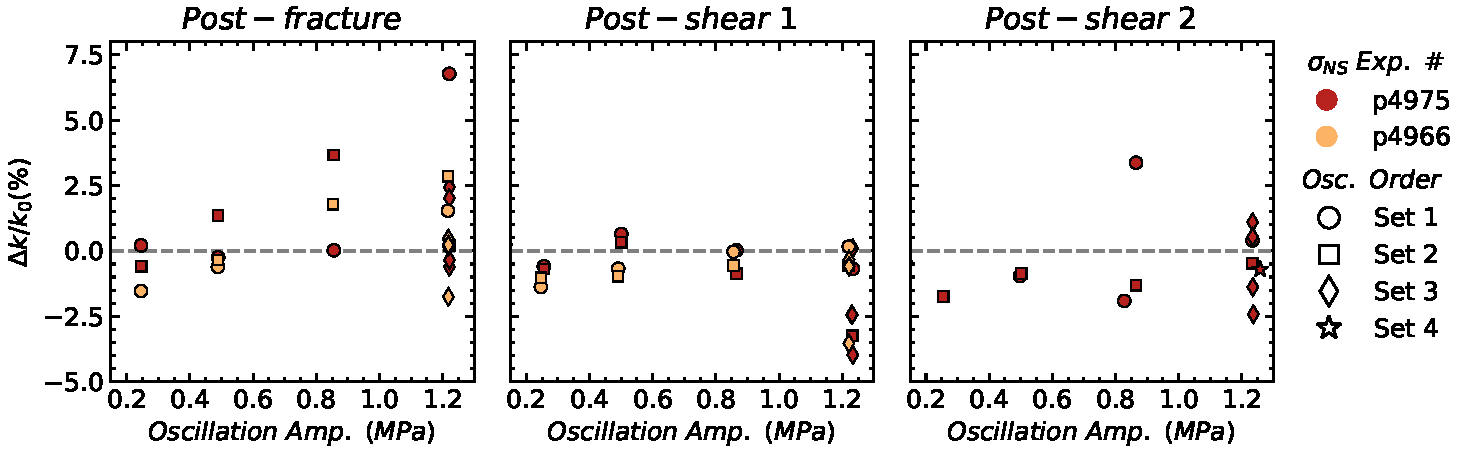
\includegraphics[width=1\columnwidth]{delk_amp_NS}
	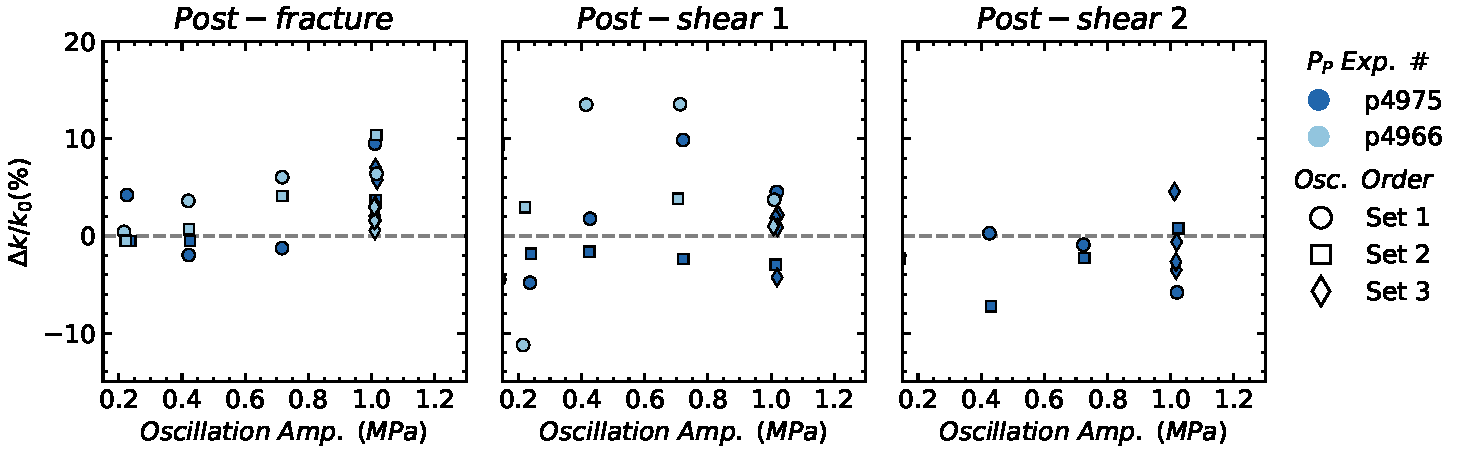
\includegraphics[width=1\columnwidth]{delk_amp_PP}
	%\enspace
	%\includegraphics[width=6cm]{post-frac_amp_array}
	\caption{Relative changes in permeability for dynamic stressing via applied normal stress (top row)  $ \sigma_{NS} $ and pore pressure (lower row) $ P_p $ at 1 Hz. Data are shown for the period just after the fracture formed (Post-fracture) and after each increment of shear. Comparing post-fracture results to post-shear we observe a general reduction of permeability enhancement via dynamic stressing with smaller values of $ \Delta k/k_0 $. Gouge generated from shear is likely clogging flow pathways along the fracture plane. The hypothesized impediment in flow for the post-shear oscillation sets causes a reduction in permeability enhancement, especially for the post-shear 2 oscillation set.}
	\label{fig:perm_ns_amp}
\end{figure*}

\clearpage

\paragraph{}
The relative change in velocity $ \Delta c/c_0 $ for the direct transmitter-receiver pair as a function of 1 Hz normal stress and pore pressure oscillation amplitudes are plotted in Figure \ref{fig:delc_ns_amp}. As expected [Riviere et. al, 2015], we observe increasing nonlinearity (more negative $ \Delta c/c_0 $) with oscillation amplitude for both normal stress and pore pressure. 

In this measure of fracture nonlinearity there is a clearer trend between oscillation order and magnitude, for this transmitter-receiver path. Normal stress oscillations for the post-fracture case exhibit less nonlinearity compared to  subsequent oscillation sets.The degree of nonlinearity from pore pressure oscillations, though linear with oscillation amplitude, remains relatively unchanged with shearing. 

The effect of shear on fracture nonlinearity is more obvious for pore pressure oscillations and rather scattered for applied normal stress oscillation sets. Interestingly, the nonlinearity relationship with amplitude barely changes with amount of shear for p4975; though for p4966,  shearing the fracture increases the nonlinearity. However, for applied normal stress successive shear scatters the trend we observe in post-fracture sets, presumably deriving from dramatic changes in asperity contacts that occur with progressive shear displacement.

\clearpage

\begin{figure*}[ht]
	\centering
	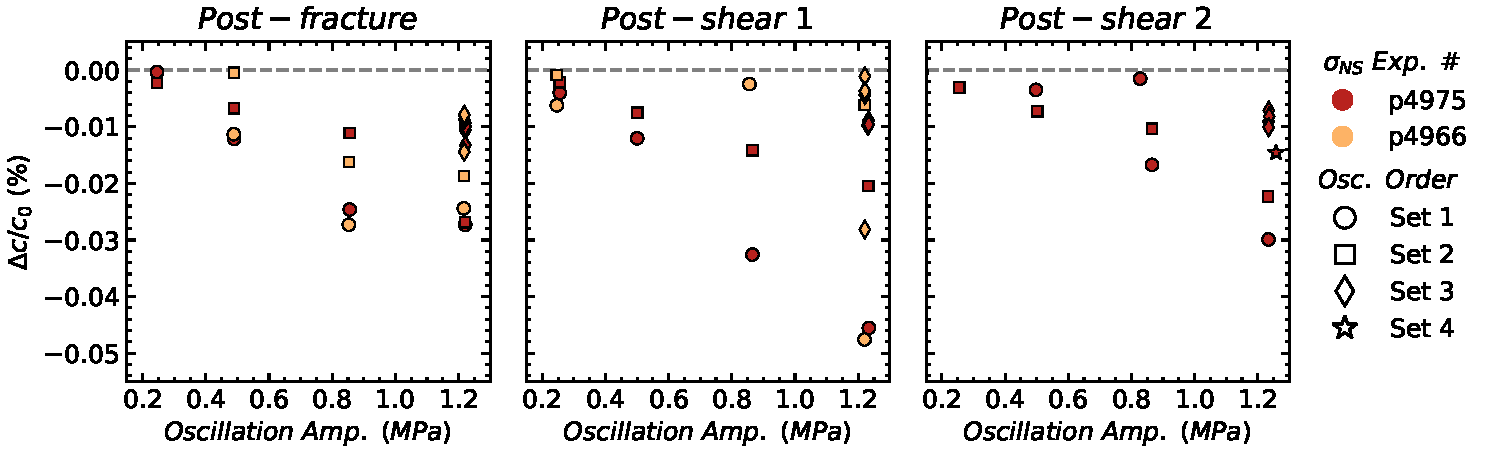
\includegraphics[width=1\columnwidth]{delc_amp_NS}
	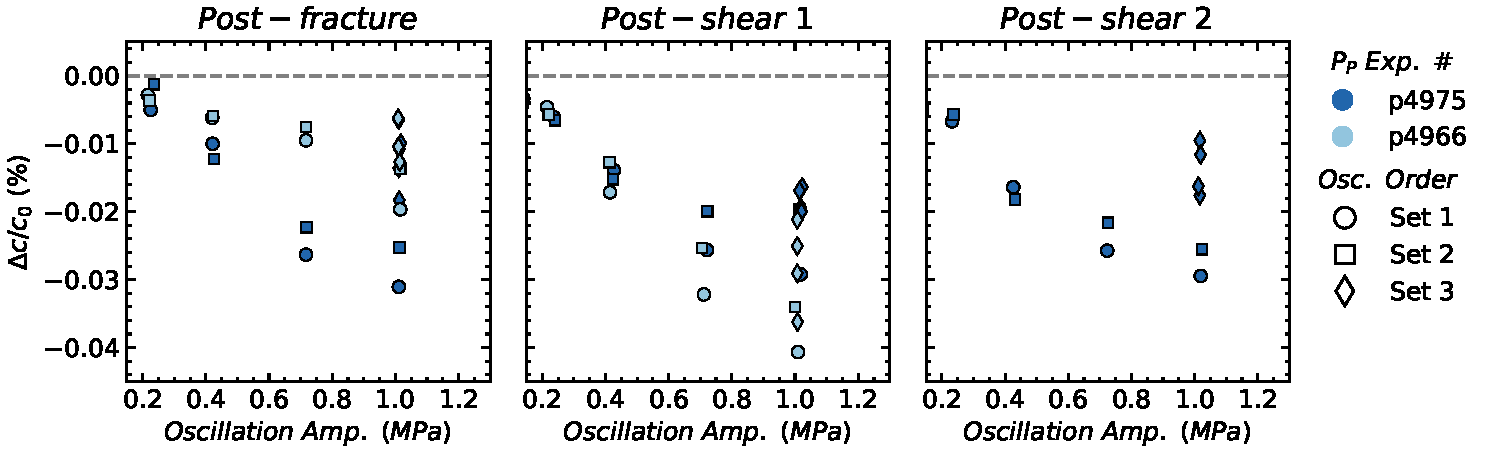
\includegraphics[width=1\columnwidth]{delc_amp_PP}
	%\enspace
	%\includegraphics[width=6cm]{post-frac_amp_array}
	\caption{ Relative changes in p-wave speed for dynamic stressing via applied normal stress (top row)  $ \sigma_{NS} $ and pore pressure (lower row) $ P_p $. Data are shown for the direct transmitter-receiver pair (see Figure 2). Note that the magnitude of $ \Delta c $  increases as a function of oscillation amplitude. Transitioning from post-fracture results to post-shear results, we observe decreased and more scattered nonlinearity.}%
	\label{fig:delc_ns_amp}
\end{figure*}

\clearpage


\subsection{Spatial Variations of the Nonlinear Elastodynamic Response}
\paragraph{}
The elastic response ($ \Delta c/c_0 $) presented in Figure \ref{fig:delc_ns_amp} corresponded to a single pair of transducers. 
% In our experiments elastic waves propagate orthogonal to the fracture plane and their amplitude, and phase depend on the fracture aperture in the wavepath. Permeability measurements comparing inlet and outlet fluid flow reveal changes in the fracture aperture across the fracture plane. 
Figure \ref{fig:delc_plots_ns} shows a coarse view of the nonlinear elastodynamic response across the fracture as a function of applied oscillation amplitude. Note that data point shape corresponds to oscillation frequencies. The direct path sensor, blue PZT in Figures \ref{fig:delc_plots_ns} -- \ref{fig:delc_plots_pp}) shows a general trend of increasing nonlinearity with stress oscillation amplitude and frequency, in both experiments. The other sensors measure more scatter and also more linearity in the case of the bottom sensor of p4975. The shearing reduces nonlinearity (direct pair) and modestly increases nonlinearity (top sensor path), but does not have an overall coherent trend for both experiments and all increments of shear.
The response to pore pressure oscillations, Figure \ref{fig:delc_plots_pp}, shows more coherent results as compared to applied normal stress. Again, there is a general trend in increasing nonlinearity with amplitude and oscillation frequency; it is interesting that the bottom receiver path exhibits markedly lower nonlinearity. Furthermore, there is much more similarity in results for the separate experiments than observed in the normal stress oscillations. Another important observation is that shearing has little effect on the magnitude of nonlinearity for pore pressure oscillations.

The scatter in these results is not unexpected given that the fracture has a heterogeneous aperture and gouge composition, especially with application of shear displacement. It is conceivable that shear increases the aperture in some locations, which could be filled with gouge material or remain empty, while other parts of the fracture aperture could be closed. These possibilities may be partially responsible for the complicated behavior we observe.

To further our understanding of the coupling between elastodynamic and hydraulic response to dynamic stressing, we investigate the spatial variations of the elastic response along the fracture by analyzing all available transmitter-receiver pairs measurement of wave velocity (Figures \ref{fig:delc_plots_ns} -- \ref{fig:delc_plots_pp}).
% We further probe this topic by determining the degree to which contact stiffness and hydraulic properties co-vary during dynamic stressing. 
Figure \ref{fig:delc_plots2} relates permeability changes $ \Delta k/k_0 $, a hydraulic measurement averaged over the fracture plane, to the change in wave velocity $ \Delta c/c_0 $ averaged across all receiver locations. The data point shapes correspond to the oscillation frequencies and their sizes correspond to oscillation amplitude. The main observation for the post-fracture oscillation sets is that relative changes in permeability and wave velocity are correlated. That is to say, larger normal stress or pore pressure oscillation amplitude and frequencies produce larger transient softening and permeability enhancement. Overall, shear weakens this relationship, reducing the amount of nonlinearity and permeability enhancement for both methods of dynamic stressing. Though, in the case of normal stress oscillations, the relationship with amplitude and frequency still exists, just the overall slope decreases due to shear displacement.

We conjecture that the nature of the correspondence between nonlinear elastodynamic and hydraulic properties of fractured rock depend not only on fracture aperture change due to stressing but also on clogging mechanisms. During both types of dynamic stressing fracture flow conduits are likely to be clogged/unclogged in a complicated fashion, resulting in mobilization of gouge material (generated from in-situ fracture and subsequent shear displacement) and permeability enhancement/reduction. This has also been in observed in previous studies of Berea sandstone (Elkhoury et al., 2011; Candela et al., 2014, 2015). However unlike in previously reported studies, we observe permeability enhancement for both normal stress and pore pressure oscillations (for amplitudes $ > 0.5 $  MPa). Thus, fracture aperture change from stressing and clogging mechanisms can not adequately explain the rich underlying physics.

%\subsection{Relative Change in Velocity and Permeability: Ray Paths}

\begin{figure*}[ht]
	\centering
	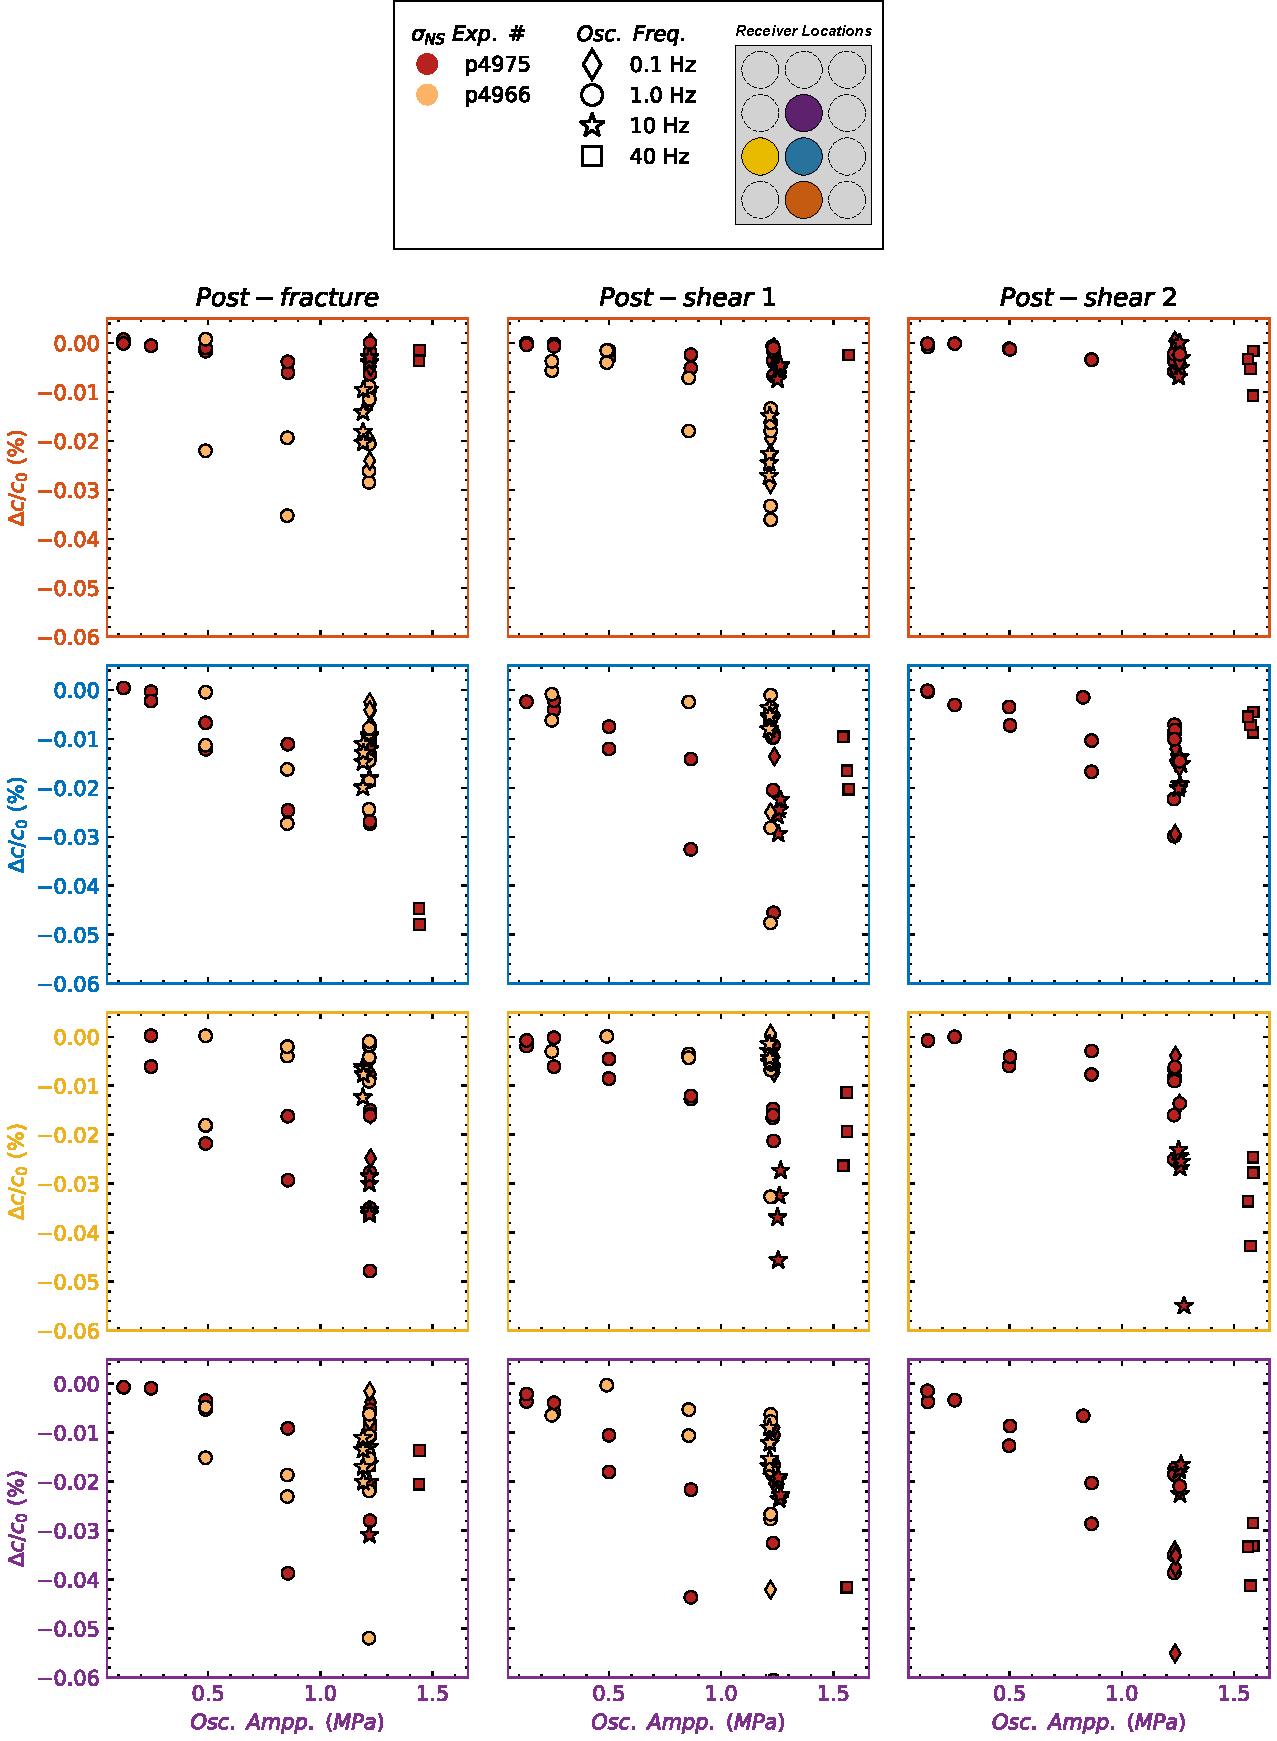
\includegraphics[width=0.9\columnwidth]{Delc_bypair_all_NS}
	\caption{Nonlinearity as a function of $ \sigma_{NS} $ oscillation amplitude for each receiver. Transitioning from post-fracture results to post-shear results, we observe decreasing nonlinearity. The plot colors correspond to PZT receiver locations. These results demonstrate the spatial variability in nonlinear elasticity across the fracture plane and furthermore shows that the two Westerly granite samples exhibit similar responses to the normal stress oscillations.  }
	\label{fig:delc_plots_ns}
\end{figure*}

\clearpage

\begin{figure*}[ht]
	\centering
	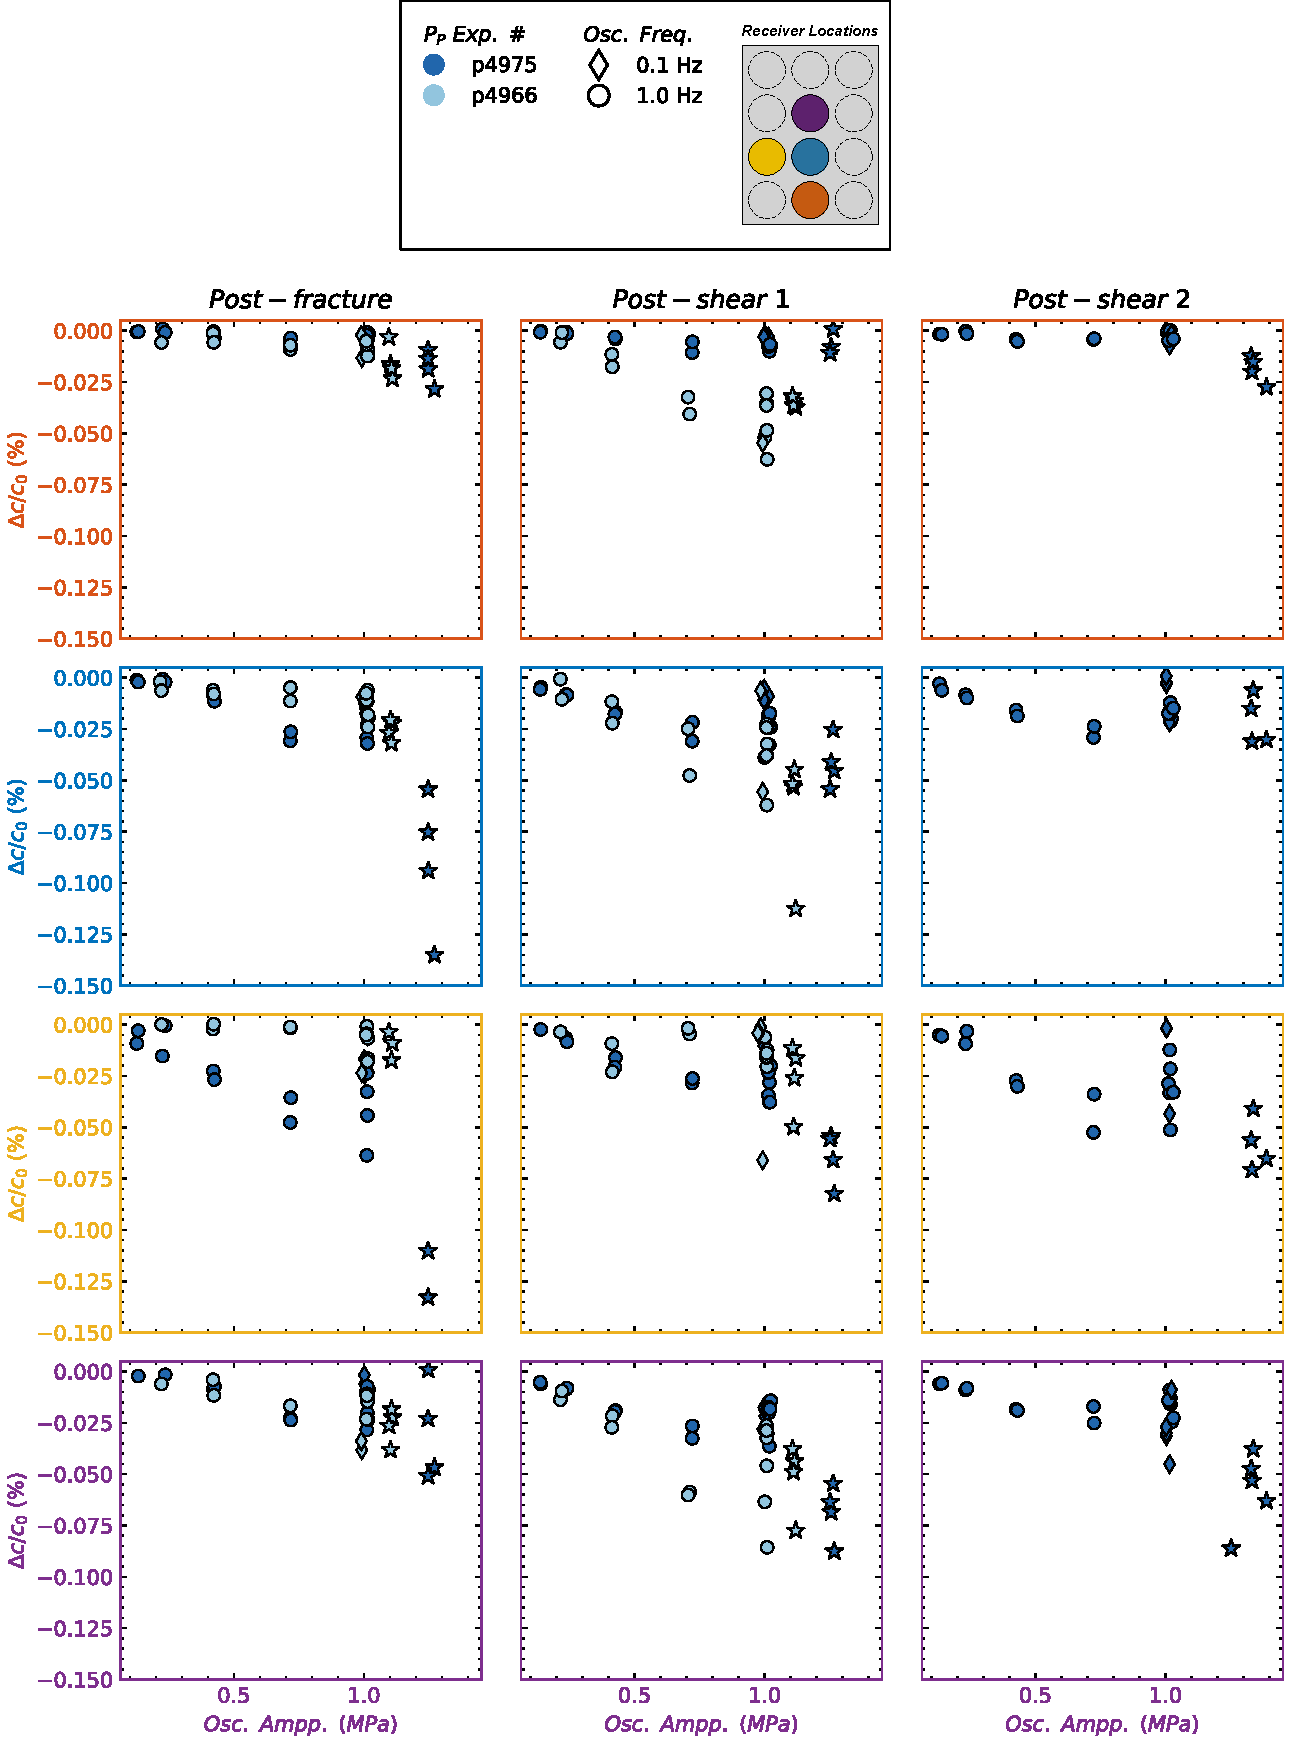
\includegraphics[width=0.9\columnwidth]{Delc_bypair_all_PP}
	\caption{Nonlinearity as a function of pore pressure oscillation amplitude for each receiver. Transitioning from post-fracture results to post-shear results, we observe decreased nonlinearity. The spatial variability shows that the pore pressure oscillations in some of the receiver locations throughout the experiments cause larger changes in elastic nonlinearity than the normal stress oscillations.}
	\label{fig:delc_plots_pp}
\end{figure*}

\clearpage


\begin{figure*}[ht]
	\centering
	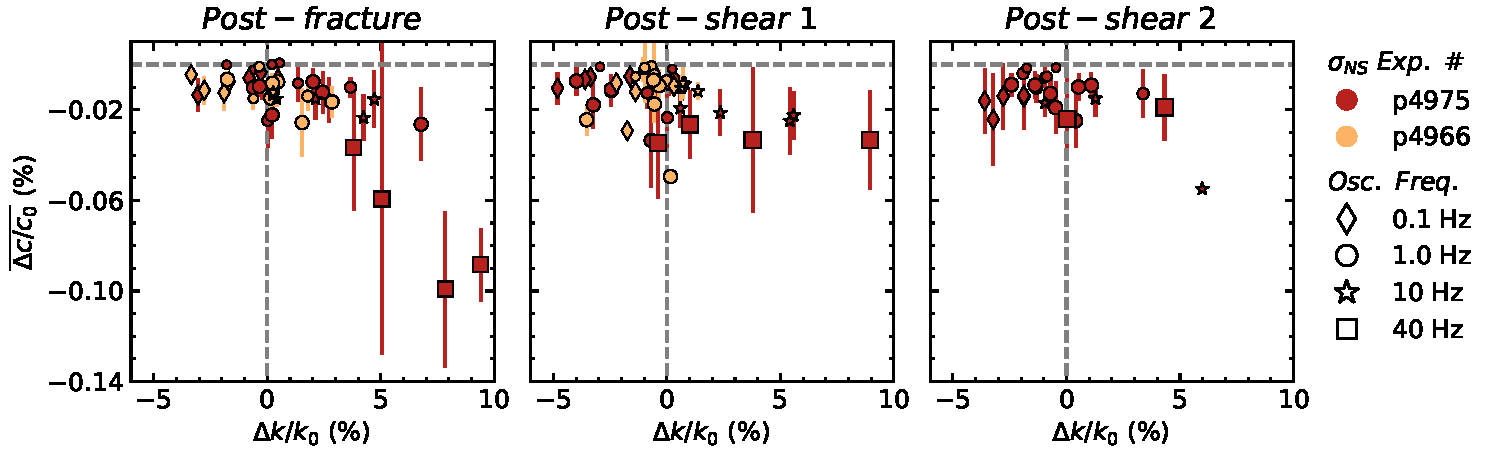
\includegraphics[width=1\columnwidth]{avgDelc_All_ampsNS}
	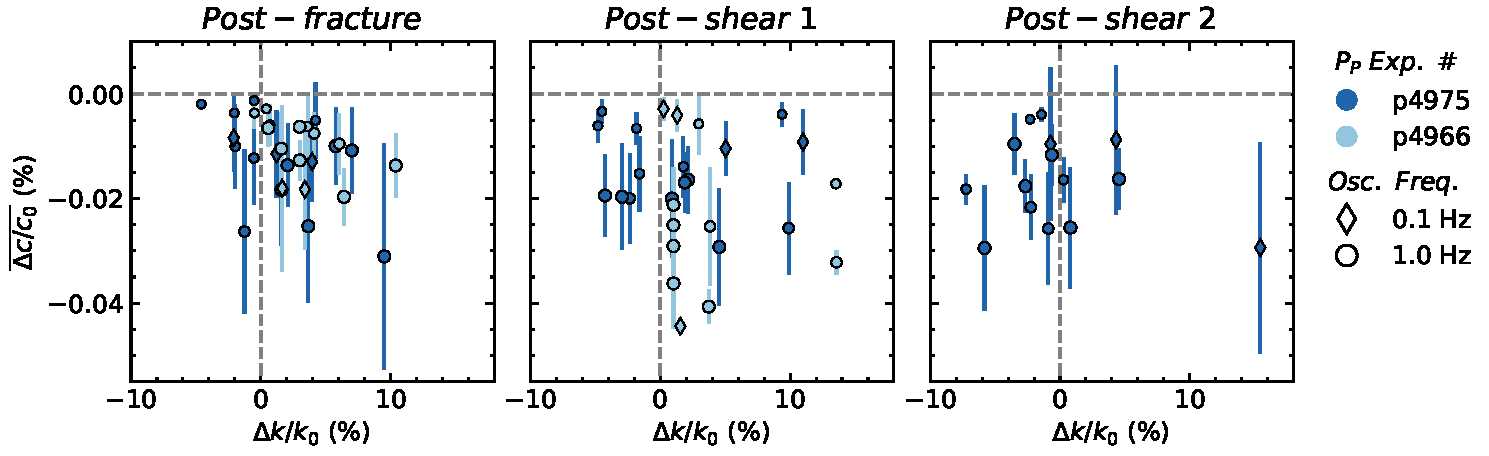
\includegraphics[width=1\columnwidth]{avgDelc_All_ampsPP}
	%\enspace
	%\includegraphics[width=6cm]{post-frac_amp_array}
	\caption{Nonlinearity as a function of permeability change for $ \sigma_{NS} $ and $ P_P $ oscillations averaged over all receivers. Data point shapes correspond to the oscillation frequencies and their sizes to amplitude. In post-fracture oscillation sets relative changes in permeability and wave velocity are correlated. That is to say, larger normal stress or Pore pressure oscillation amplitude and frequencies produce larger transient softening and permeability enhancement. Overall, shear weakens this relationship, reducing the amount of nonlinearity and permeability enhancement for both methods of dynamic stressing. }
	\label{fig:delc_plots2}
\end{figure*}

\clearpage

\subsection{Wave Velocity Modulation}
\paragraph{}
The direct effect of dynamic stressing is an instantaneous modulation in wave velocity at harmonic frequencies of the driving frequency. We denote the mean velocity amplitude as $ dc $ (e.g., Figure 5). The relative change in average velocity oscillations $ dc/c_0 $ is a proxy for the nonlinear parameter $ \beta $, estimated from the second harmonic (e.g., [Rivière et al., 2013, 2015]). We observe a monotonic relationship between the magnitude of $ dc/c_0 $ and oscillation amplitude for both rock samples (Figure \ref{fig:dc_plots2}).

There is a consistent trend that subsequent oscillation sets decrease the magnitude of nonlinearity of $ dc/c_0 $ for normal stress modulation. Pore pressure oscillations exhibit little to no change through subsequent repetitions, except for larger driving amplitudes.  Shearing the fracture decreases the measured nonlinearity, especially for experiment p4966 (Figure 15). This is also observed for pore pressure oscillations in sample p4966, but p4975 exhibits little to no change in $ dc/c_0 $ nonlinearity after the first shear increment. Then, after the second shear, pore pressure oscillations interestingly increases the nonlinearity. We posit that the two types of dynamic stressing activate two different mechanisms: (1) opening/closing of pore throats from normal stress oscillations and (2) directly dislodging and mobilizing fines along the fracture from pore pressure oscillations. This is consistent with our observations of other nonlinearity parameters. 
\clearpage

\begin{figure*}[ht]
	\centering
	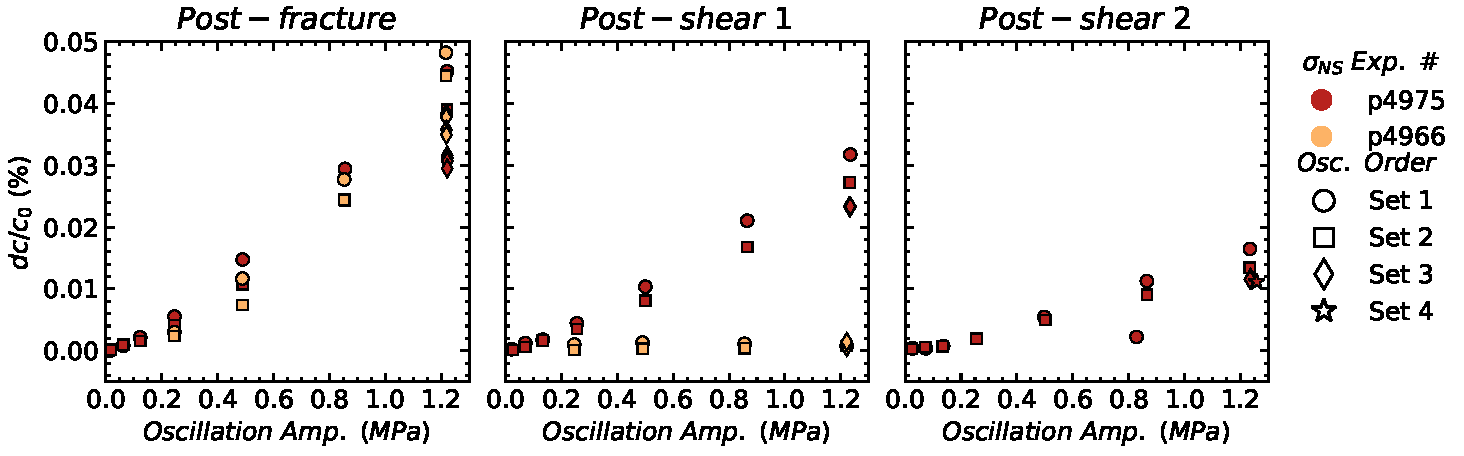
\includegraphics[width=1\columnwidth]{dc_amp_NS}
	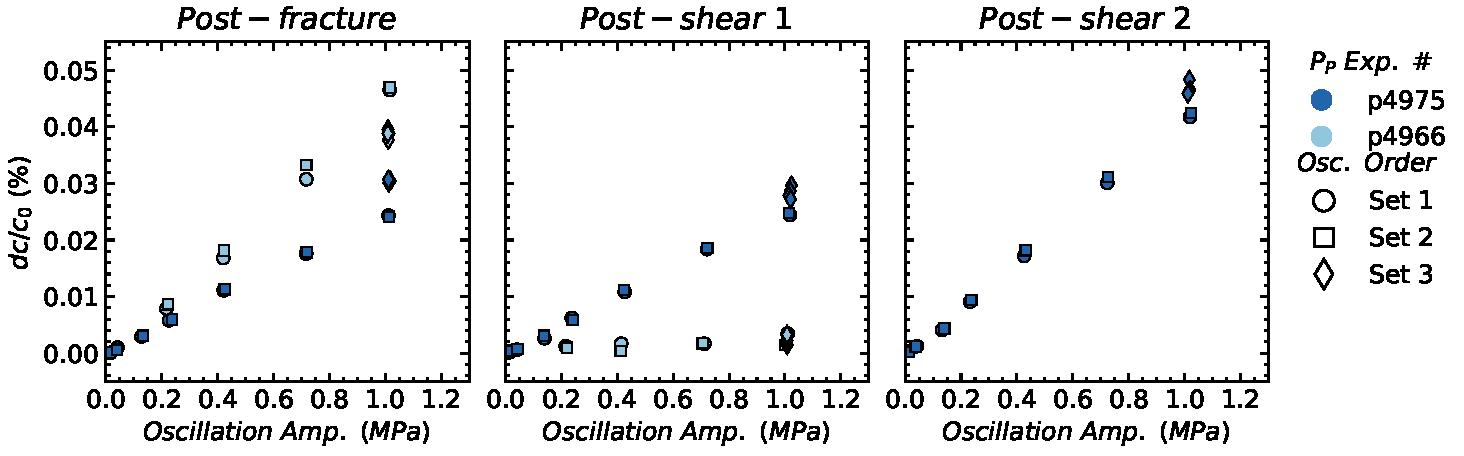
\includegraphics[width=1\columnwidth]{dc_amp_PP}
	%\enspace
	%\includegraphics[width=6cm]{post-frac_amp_array}
	\caption{Velocity amplitude modulation averaged over all receivers ($ dc/c_0 $) as a function of normal stress and Pore pressure oscillations. There is a systematic reduction in $ dc/c_0 $ with accumulated shear for normal stress oscillations and there is very little variation in the oscillation order. The results from pore pressure oscillations in p4966 tell a similar story as the normal stress oscillations, but the pore pressure oscillations in p4975 show no change from post-fracture to post-shear 1 and an increase in $ dc/c_0 $ from post-shear 1 to 2.}
	\label{fig:dc_plots2}
\end{figure*}
\clearpage

\subsection{Permeability and Wave Velocity Recovery from Dynamic Stressing}
\paragraph{}
% Dynamic stressing in the subsurface could Field scale observations of subsurface water pressure 
% Oscillations in pore pressure resulting from the passage of seismic waves could drive a flow that dislodges fine particles clogging pore throats, which would generate dynamic permeability enhancement (Brodsky et al., 2003, Roberts, 2005, Elkhoury et al., 2011). In this case, the gradual recovery of permeability to its initial state could be related to re-clogging of pore throats via slow migration of fine particles after the dynamic stimulation.
% During the oscillations, the fines initially plugged in the pore throats (or between fracture asperities) are flushed, producing the direct permeability enhancement observed in our experiments.
% Prior laboratory experiments show that pore pressure oscillations can produce permeability increases in lithified rock that: (1) scale with amplitude of the perturbations and (2) persist long after the oscillations cease (Elkhoury et al., 2011). Here we expand on existing works and report on a systematic set of experiments to explore the evolution of permeability for intact and fractured rock for a range of water solution chemistries and flow rates.
% Our experimental set-up is designed to separate the three major candidate mechanisms: (i) dislodging of fines by oscillatory flow followed by the progressive re-clogging of pore throats via slow migration of fines, (ii) damage followed by micro-fracture healing, (iii) direct increase in aperture followed by poroelastic drainage resulting in prolonged fracture opening. We impose dynamic stresses via pore fluid pressure oscillations and analyze the resulting evolution of permeability. 
The long term evolution of permeability and wave velocity reveal the extent to which fines are transported along the fracture and how fracture asperities recover from dynamic stresses. We observe that trends, particularly in experiment p4975, where the slope of the permeability recovery linearly increases with normal stress and pore pressure oscillations, see insets of Figure \ref{fig:k_recov}. These results suggest that for normal stress oscillations larger amplitude oscillations open the fracture more, allowing for fines to unclog and migrate along the fracture. Similarly, large amplitude pore pressure oscillations are more effective in mobilizing the fines, thus allowing for a quicker recovery to its initial state. Furthermore, there is little variability in the order of oscillation for both stimulation methods. 
\paragraph{}
Shearing the fracture consistently slows the permeability recovery after normal stress oscillations, but results in quicker permeability rates in response to pore pressure oscillations, see \textit{Post - Shear 1} and \textit{2} from Figure \ref{fig:k_recov}. This suggests that normal stress oscillations (opening and closing of pore throats) become less effective in mobilizing fines and the fracture asperities are permanently damaged/altered, so the permeability cannot recover to initial pre-oscillation state. Though there is an increase accumulation of fines from shearing, the permeability recovers more quickly in response to pore pressure oscillations. We posit that the wear material undergoes comminution from subsequent shearing and normal stress oscillations, is transported along the fracture during the pore pressure oscillations, and then the permeability more quickly recovers from the transient.

\clearpage

\begin{figure*}[ht]
	\centering
	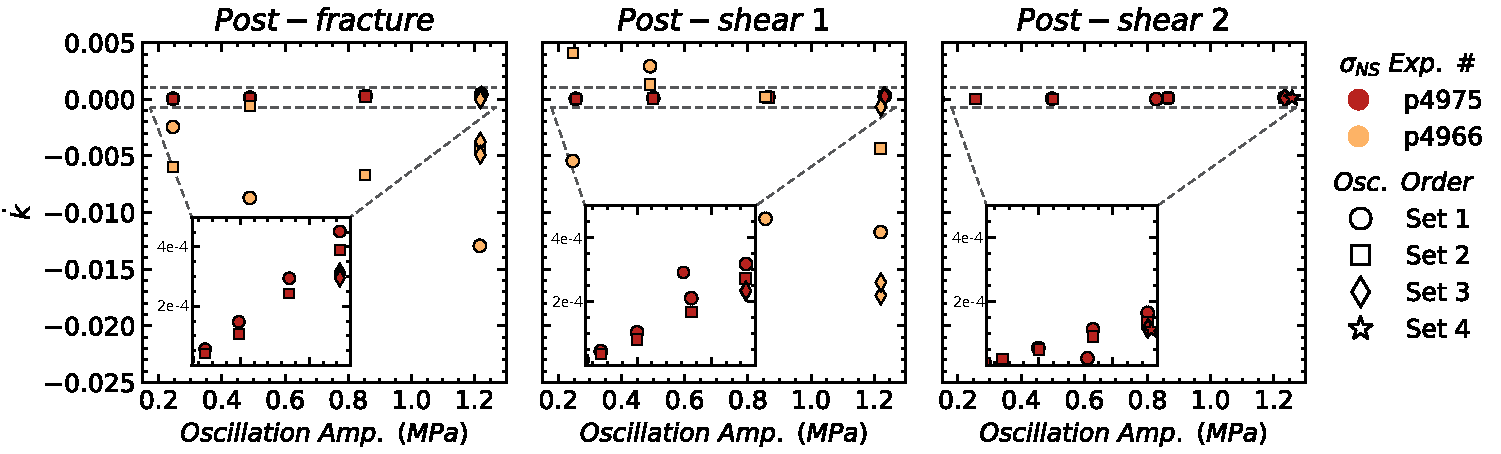
\includegraphics[width=1\columnwidth]{k_recov_amp_NS}
	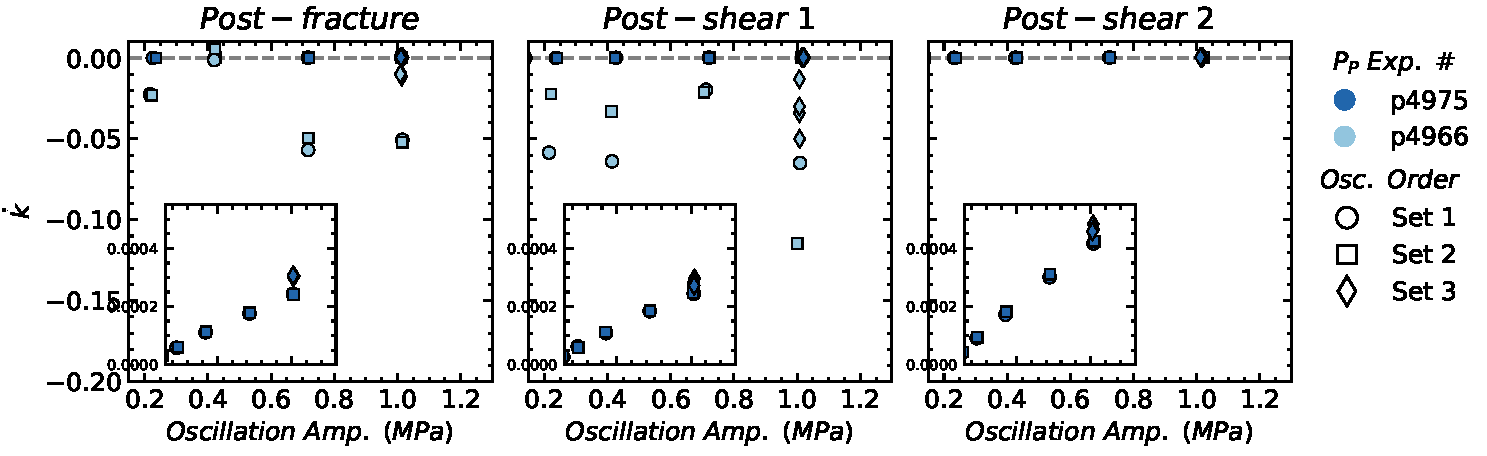
\includegraphics[width=1\columnwidth]{k_recov_amp_PP}
	%\enspace
	%\includegraphics[width=6cm]{post-frac_amp_array}
	\caption{Permeability recovery $ \dot k $ as a function of applied stress oscillations for $ \sigma_{NS} $ and $ P_P $. Data point shapes indicate oscillation order. Recovery rate $ \dot k $ linearly increases with oscillation amplitude for both $ \sigma_{NS} $ and $ P_P $ oscillations in p4975. Furthermore, subsequent shearing results in slower $ \dot k $ for $ \sigma_{NS} $ oscillations, but $ \dot k $ increases for $ P_P $ oscillations. }
	\label{fig:k_recov}
\end{figure*}
\clearpage

\paragraph{}
The wave velocity recovery rate $ \dot c $ for the direct transmitter-receiver pair as a function of 1 Hz normal stress and pore pressure oscillation amplitudes are plotted in Figure \ref{fig:c_recov}. We observe faster recover with oscillation amplitude for both normal stress and pore pressure. In the post -- fracture phase, there is a noticeable effect of order of $ \sigma_{NS} $ oscillations on recovery rate; later oscillations exhibit smaller magnitude of $ \dot c$, which demonstrates detectable damage to the fracture asperities from the first oscillation set.  

\paragraph{}
The effect of shear on fracture $ \dot c $ is decrease in the magnitude of recovery rate and a flattening of the relationship between $ \dot c $ and oscillation amplitude for both perturbation methods. There is perhaps a complex effect from deformation of fracture asperities and the granular wear material that inhibit the recovery from the transient response to dynamic stressing.  

\clearpage

\begin{figure*}[ht]
	\centering
	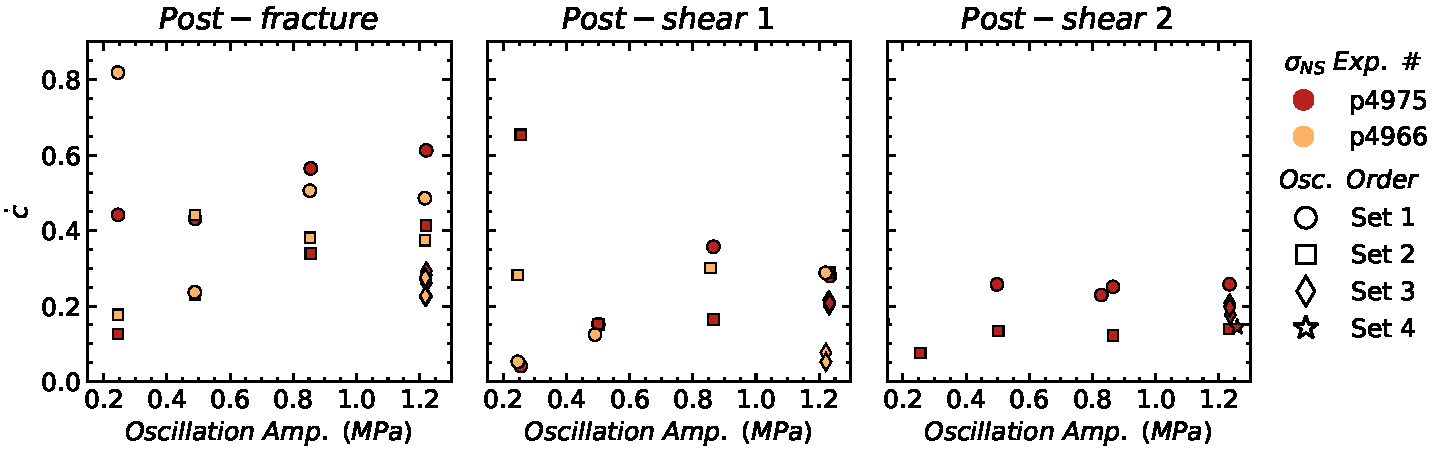
\includegraphics[width=1\columnwidth]{c_recov_amp_NS}
	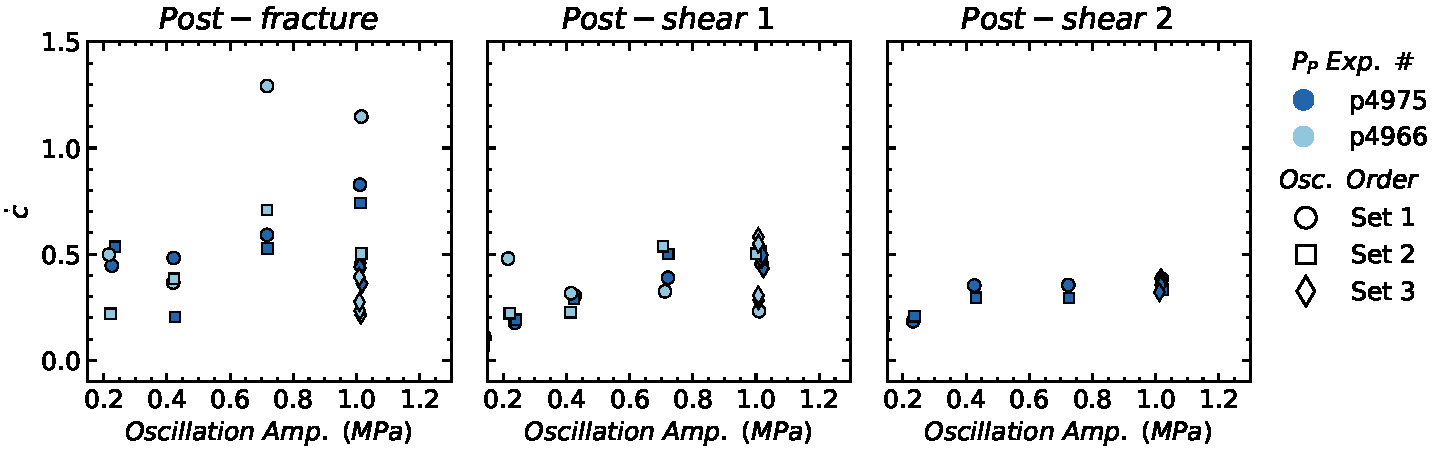
\includegraphics[width=1\columnwidth]{c_recov_amp_PP}
	%\enspace
	%\includegraphics[width=6cm]{post-frac_amp_array}
	\caption{Wave velocity recovery $ \dot c $ for direct-path receiver as a function of applied stress oscillations for $ \sigma_{NS} $ and $ P_P $. Data point shapes oscillation order. The recovery rate $ \dot c $ modestly increases with both $ \sigma_{NS} $ and $ P_P $. Shearing decreases $ \dot c $ and flattens after the second shear displacement. }
	\label{fig:c_recov}
\end{figure*}

\clearpage

\paragraph{}
Figure \ref{fig:avg_recov_plots} relates permeability changes $ \dot k $, a hydraulic measurement across the fracture, to the wave velocity recovery rate $ \dot c $ averaged over all receiver locations. The main observation from p4975 is linear relationship between $ \dot c $ and $ \dot k $ for both normal stress and pore pressure oscillations in the post -- fracture phase. Also, there is some scaling of the magnitude of $ \dot k$  with  $ \sigma_{NS}$ oscillations frequency.  Overall, shearing the fracture weakens this relationship for normal stress oscillations, but enhances it for pore pressure oscillations.

\clearpage

\begin{figure*}[ht]
	\centering
	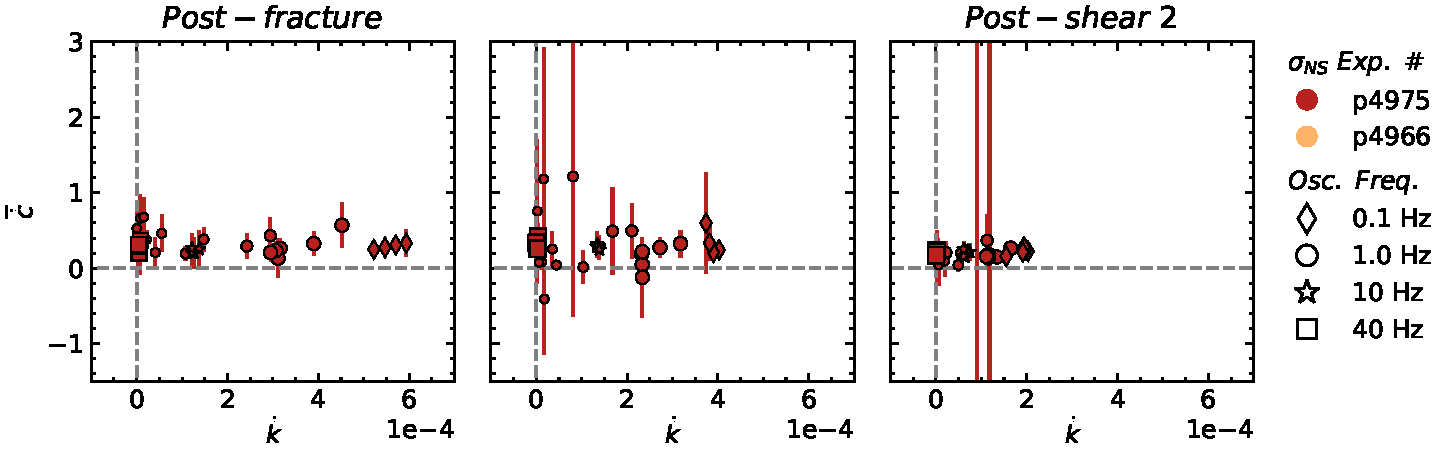
\includegraphics[width=1\columnwidth]{avg_recov_All_ampsNS}
	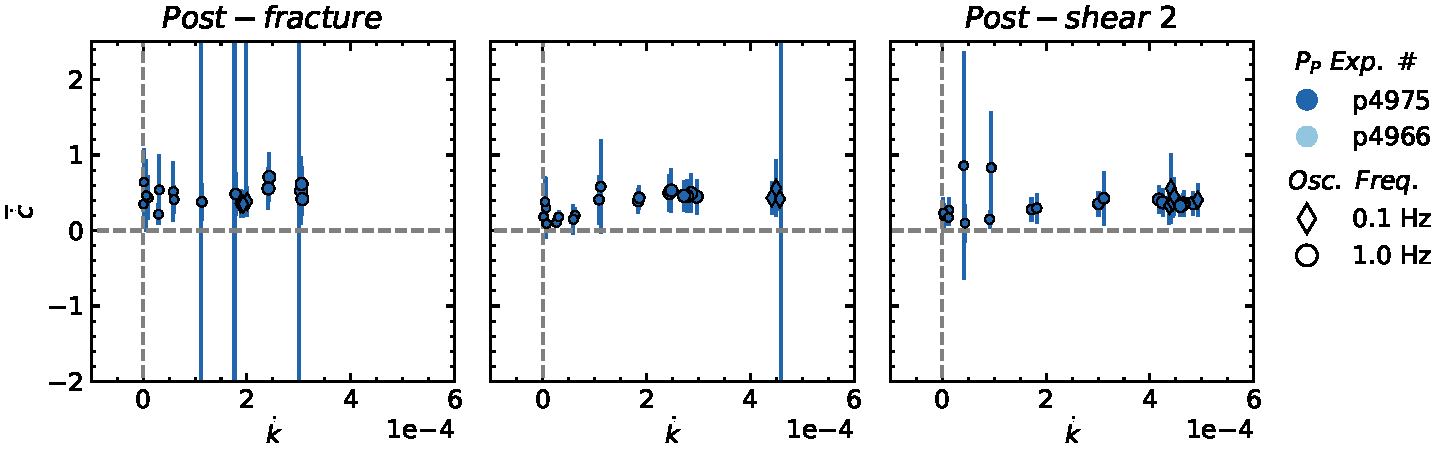
\includegraphics[width=1\columnwidth]{avg_recov_All_ampsPP}
	%\enspace
	%\includegraphics[width=6cm]{post-frac_amp_array}
	\caption{Wave velocity recovery rate $ \dot c $ as a function of permeability recovery rate $ \dot k$ for $ \sigma_{NS} $ and $ P_P $ oscillations averaged over all receivers. Data point shapes correspond to the oscillation frequencies and their sizes to amplitude. In post-fracture oscillation sets high frequency and large amplitude oscillations yield faster recovery rates for both velocity and permeability. The predominant effect of shearing is a significant reduction in $ \dot k $ for $ \sigma_{NS} $ oscillations, but increases for  $ P_P $ oscillations.}
	\label{fig:avg_recov_plots}
\end{figure*}

\clearpage

%--------------------------------------------------------------------------
%CONCLUSION
%--------------------------------------------------------------------------

\section{Conclusions}
\paragraph{}
We  conducted lab experiments to determine the effects of dynamic stressing and shearing on elastodynamic and hydraulic properties of fractured rock. Processes controlling fluid flow in reservoirs, subsufrace waste disposal, and hydrocarbon production derive from a complex interplay of these properties. Monitoring in-situ fractures with active source ultrasonic transmission and fluid permeability during two modes of dynamic stressing reveals the complex relation between elastodynamic and hydraulic properties. 

In response to oscillations of effective normal stress Westerly granite samples exhibit characteristic transient softening, velocity fluctuations, and slow recovery, informing us about the microstructure and contact mechanics. We observe that large amplitude and high frequency oscillations generally increase permeability, with pore pressure oscillations producing the largest enhancement of permeability. Furthermore, we document spatial variability in elastodynamic properties across the fractures, revealing the effect of variations in fracture aperture and contact stiffness. Shearing generally decreases this nonlinearity parameter for both oscillation modes.
We currently do not fully understand the underlying physics of how fracture asperity and aperture changes from dynamic stressing and clogging mechanisms account for these results. Our observations do suggest that the two types of dynamic stressing activate two different mechanisms; aperture change dominates during applied normal stress oscillations and unclogging dominates during pore pressure oscillations. 

Future experiments with pre-fractured samples will include characterization of surface roughness with high-resolution profilometry to better constrain the underlying mechanics of aperture and permeability change. Furthermore, we will develop methods to collect fine gouge material generated from in-situ fracturing and shearing in the downstream pore pressure lines in an attempt to quantify the degree to which unclogging mechanisms are responsible for the results we observe.
\clearpage





%--------------------------------------------------------------------------
%SUPPLEMENTAL
%--------------------------------------------------------------------------

\newcommand{\beginsupplement}{%
	%	\setcounter{table}{0}
	%	\renewcommand{\thetable}{S\arabic{table}}%
	\setcounter{figure}{0}
	\renewcommand{\thefigure}{S\arabic{figure}}%
}

\beginsupplement
\section{Supplemental}
\label{Supp}

\begin{figure*}[ht]
	\centering
	%	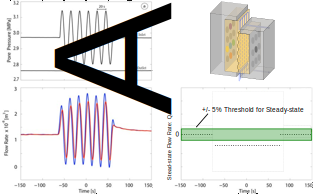
\includegraphics[width=1.0\columnwidth]{PpFlow_fig_v1}
	%	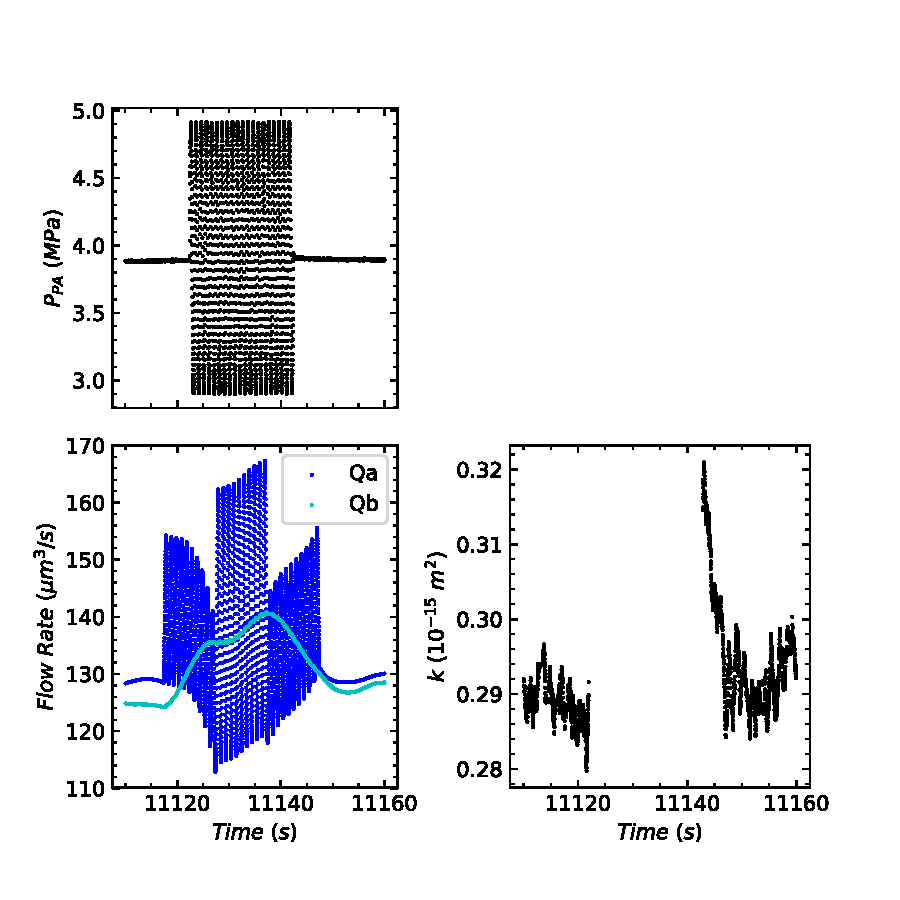
\includegraphics[width=0.8\columnwidth]{permCalcPlots_p4975_run3b_1Hz}
	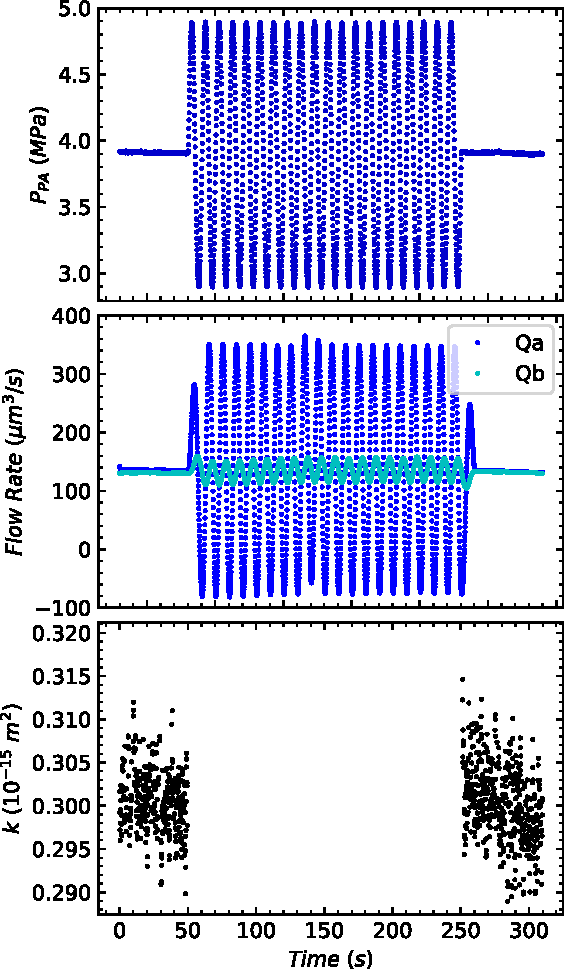
\includegraphics[width=0.4\columnwidth]{permCalcPlots_tall_p4975_run3b_1Hz}
	\caption[]{Example of dynamic stressing and the corresponding flow rate measurements for a set of pore pressure oscillations in experiment p4975. Note that the plots (a) and (b) are decimated for clarity. (a) Imposed pore pressure oscillation at inlet and fixed pore pressure at the outlet. Pressure conditions before and after the oscillations are identical. (b) Measured flow rates at the fracture inlet (blue line) and outlet (red dashed line). Notice the small time lag ($\leq$ 2 s) between the maxima of the inlet and outlet flow rates. (c) Permeability at steady-state and during the pore pressure oscillation. In the calculation of permeability we impose a threshold between the flow rates to ensure steady-state flow ($Q_{A} - Q_{B}  \leq 5 \% $). It is reasonable to assume that even at relatively low frequency oscillations, there is effectively no steady-state flow during the imposed oscillations.}
	\label{fig:perm_calc}
\end{figure*}

\textcolor{red}{We measure the effective permeability, ka, by calculating the flow rate over a 2 s window. For pore pressure oscillations, we start 10 s after the oscillation to ensure that permeability measurement is not affected by the Pp oscillation and/or by storage effects. Need to annotate Flow Rate with lines indicating the +- 5\%}

\newpage


%\begin{figure}[ht]
%	\centering
%	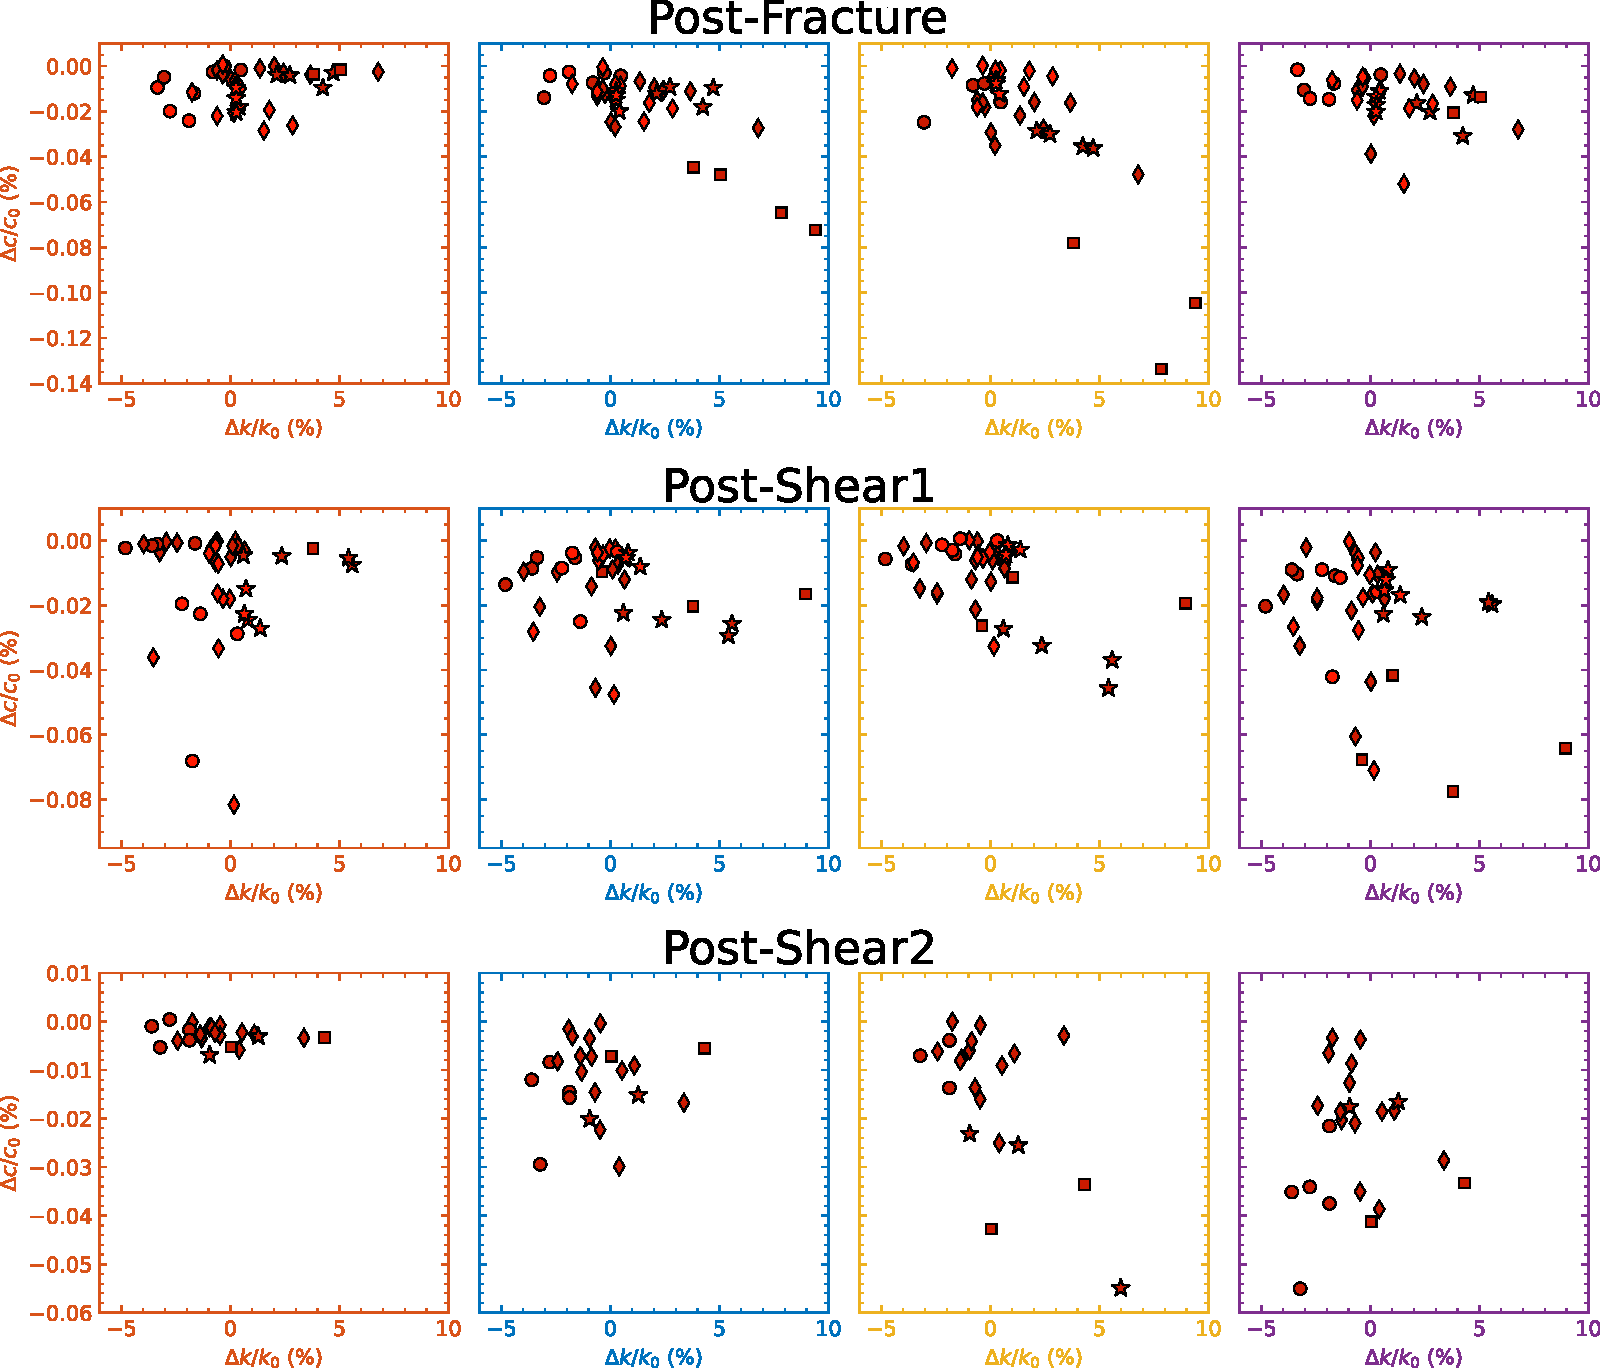
\includegraphics[width=1\columnwidth]{Delc_all_NS_all}
%	%\enspace
%	%\includegraphics[width=6cm]{post-frac_amp_array}
%	\caption{Nonlinearity as a function of permeability change for $ \sigma_{NS} $ oscillations for each receiver. Transitioning from post-fracture results to post-shear results, we observe decreased nonlinearity and permeability enhancement. This is probably related to clogging mechanisms.}%
%	\label{fig:delc_plots_ns}
%\end{figure}
%
%\newpage
%
%\begin{figure}[ht]
%	\centering
%	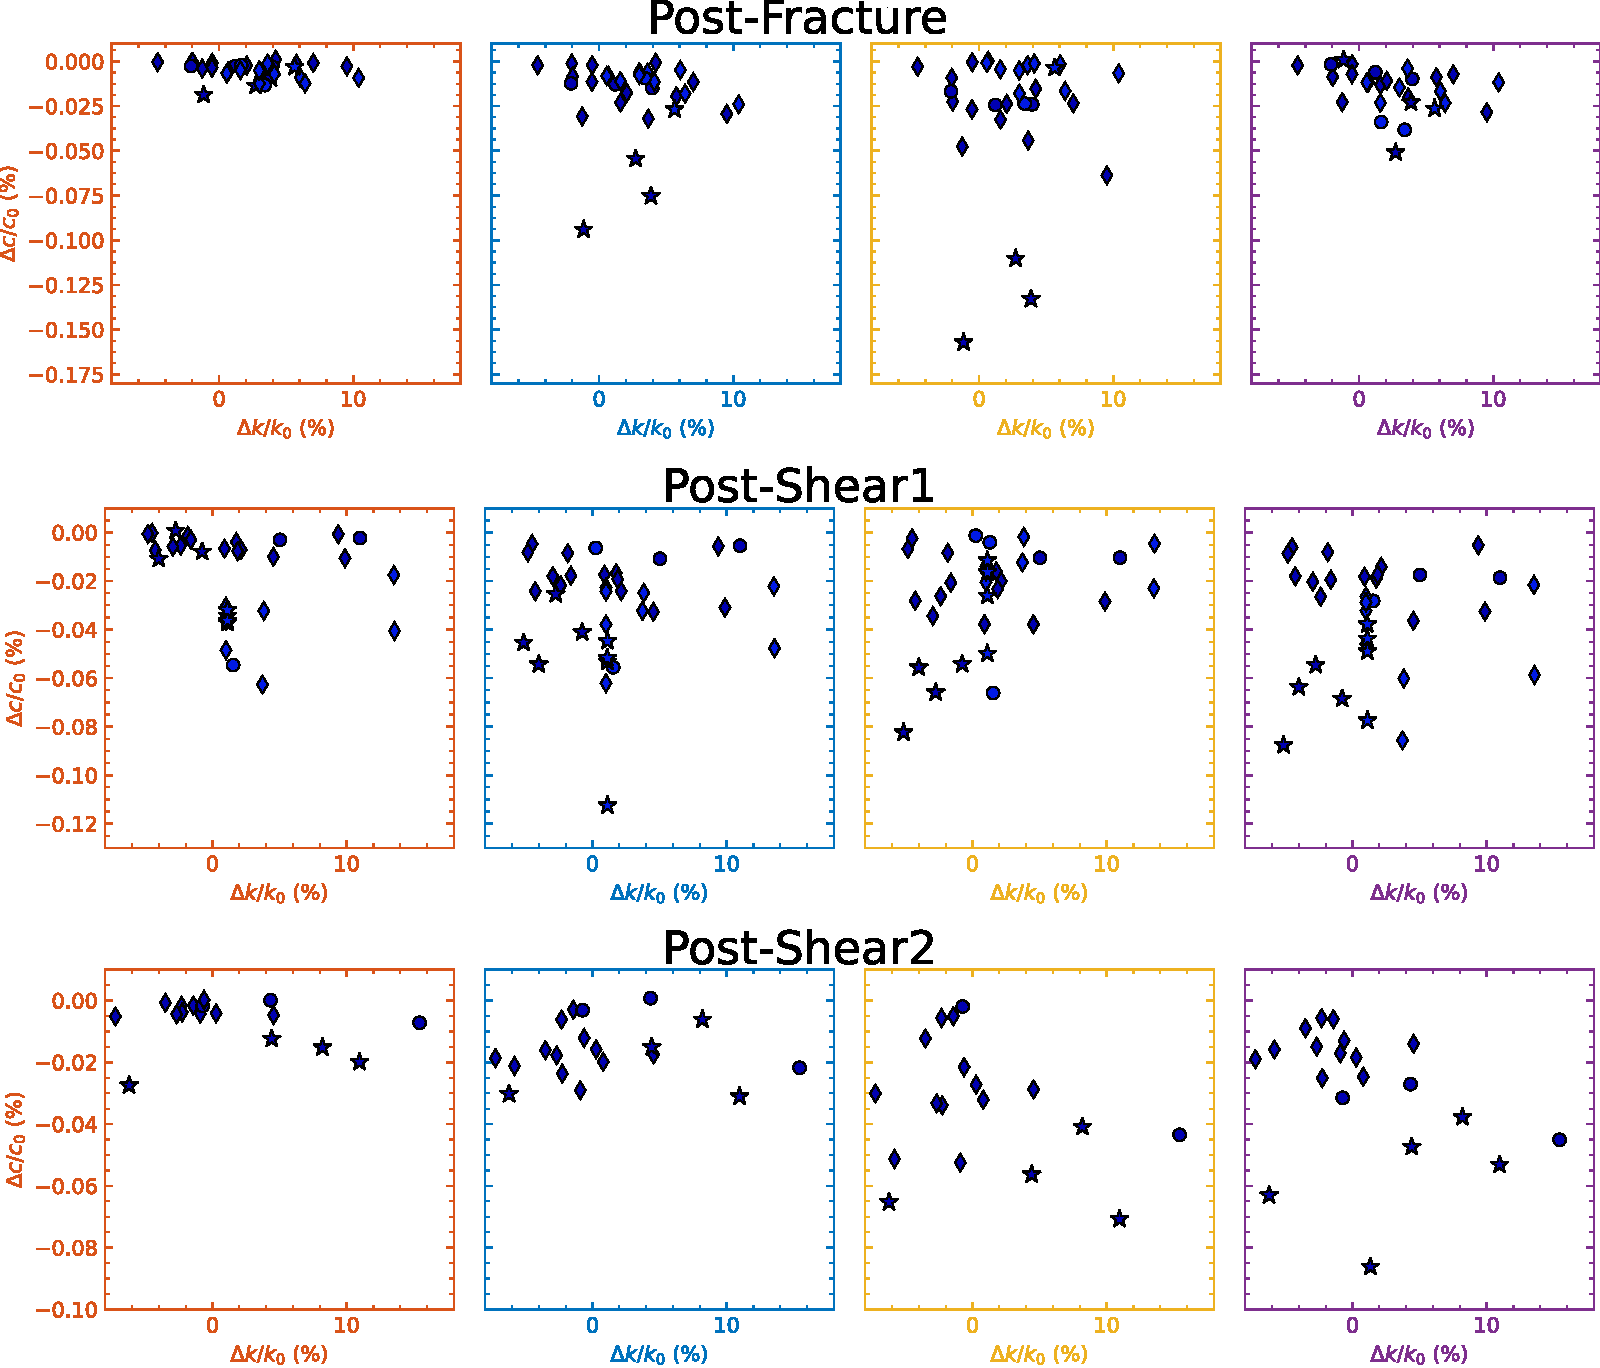
\includegraphics[width=1\columnwidth]{Delc_all_PP_all}
%	%\enspace
%	%\includegraphics[width=6cm]{post-frac_amp_array}
%	\caption{Nonlinearity as a function of permeability change for $ P_P $ oscillations for each receiver.}
%	\label{fig:delc_plots_pp}
%\end{figure}

\newpage

\begin{figure}[ht]
	\centering
	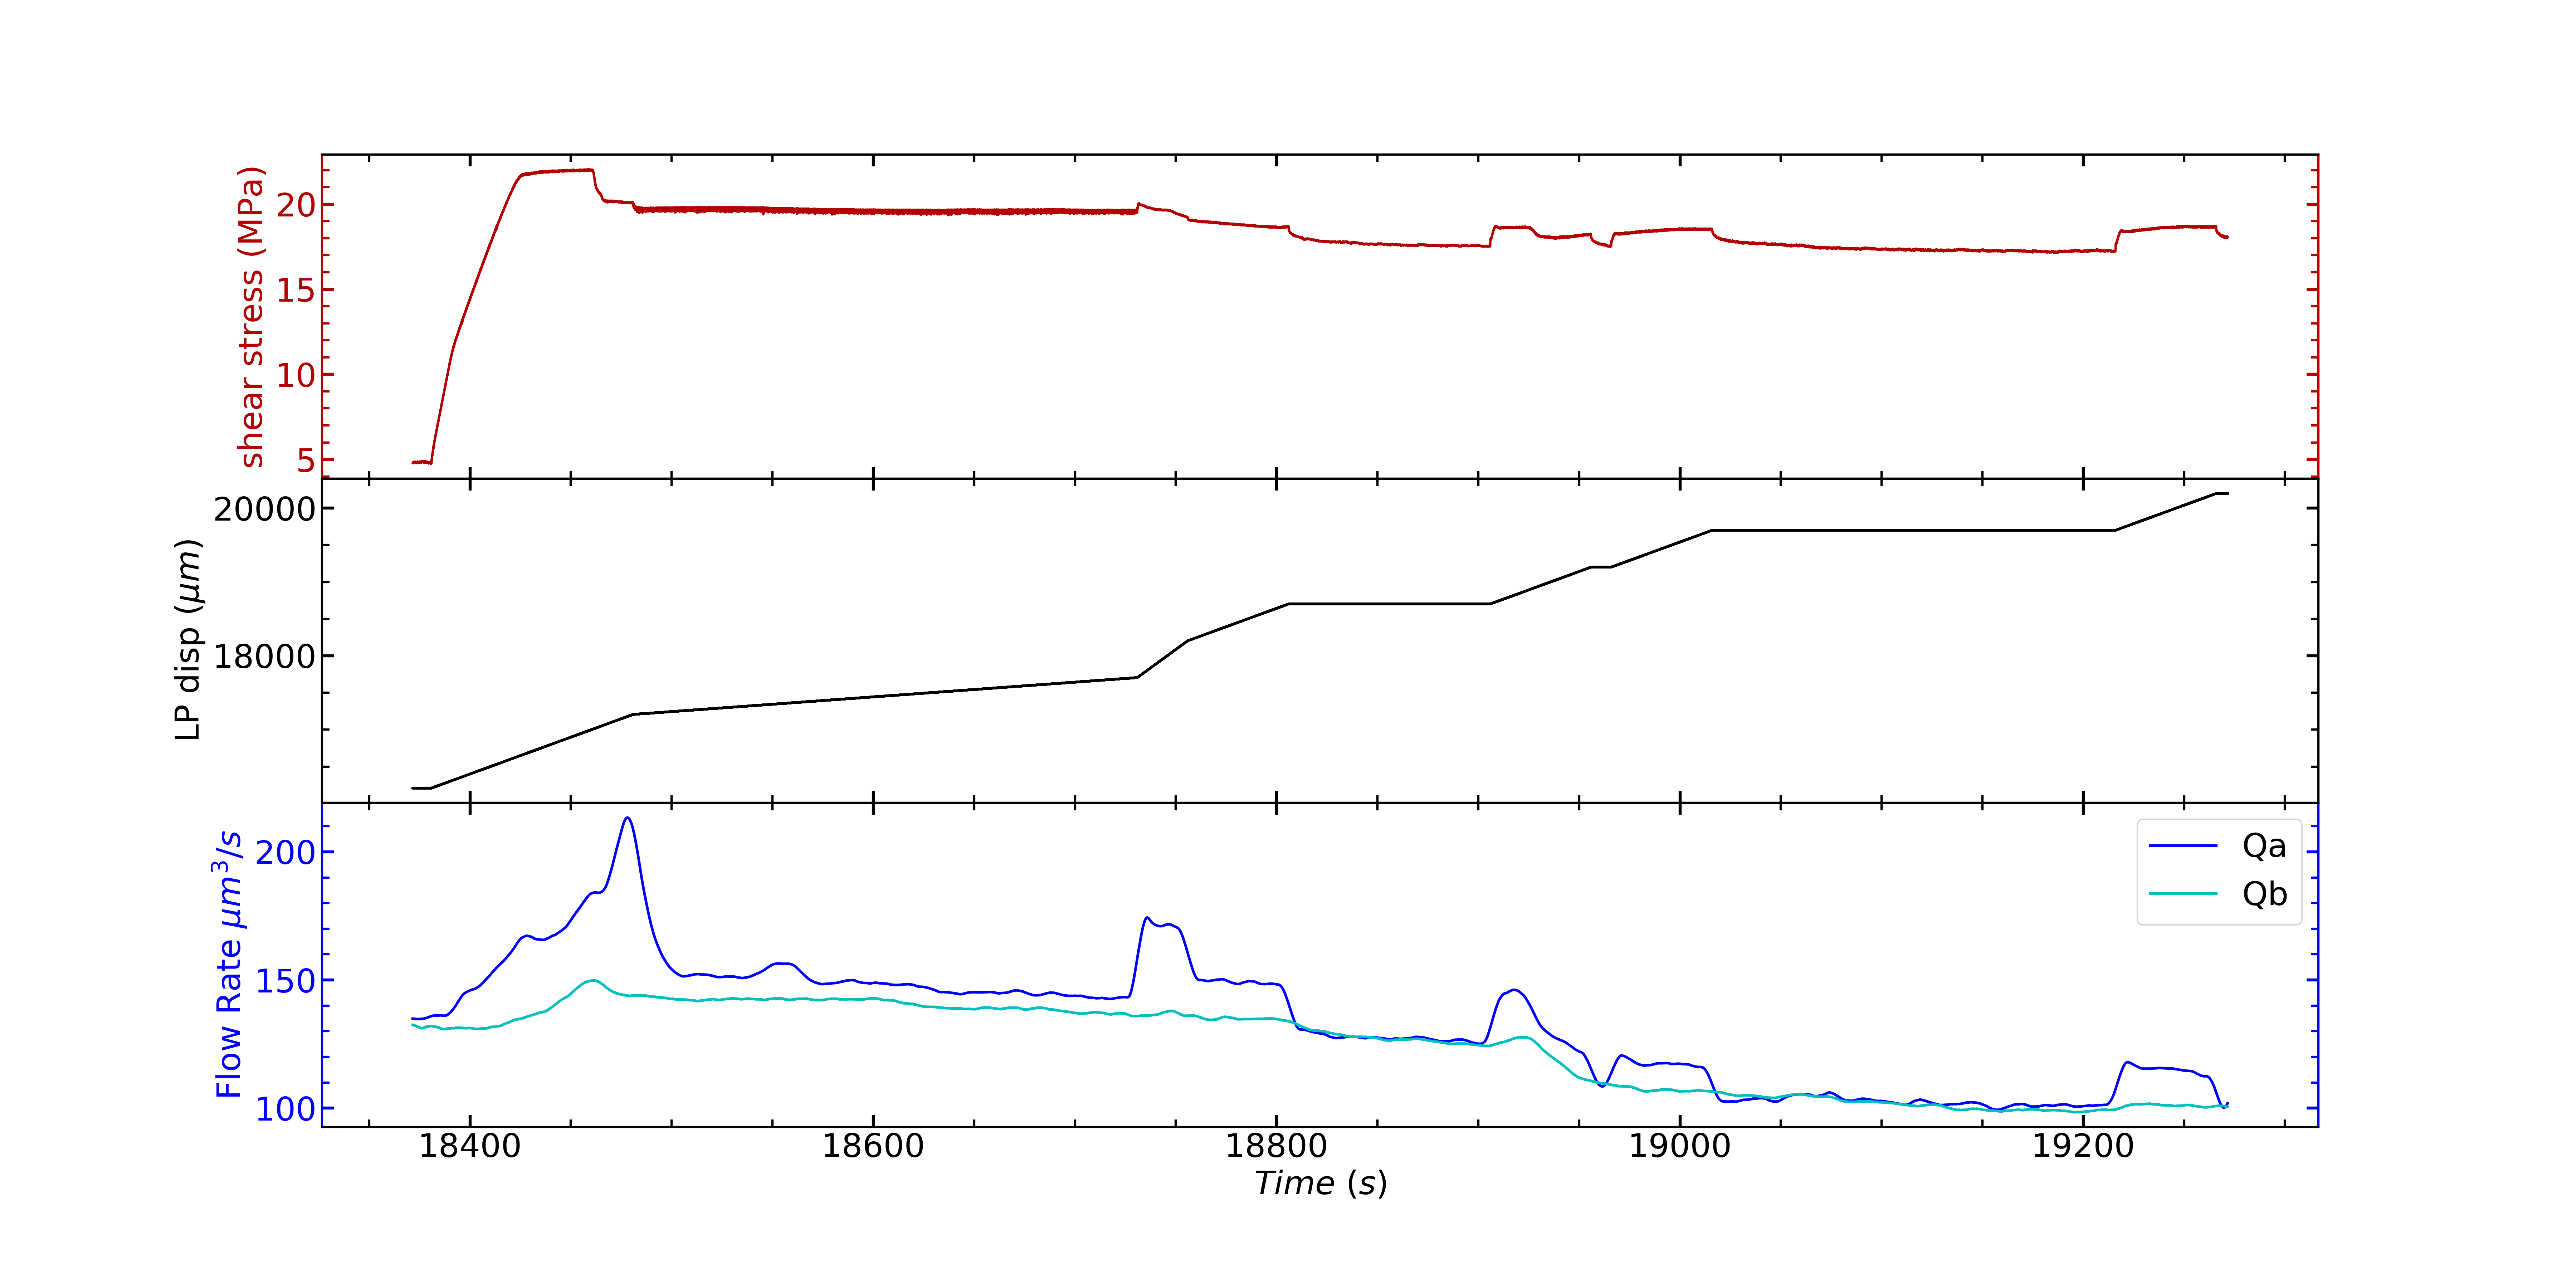
\includegraphics[width=1\columnwidth]{Shearing_p4975_shr1}
	\caption{First shearing for p4975.}
	\label{fig:shr1_p4975}
\end{figure}

\newpage

\begin{figure}[ht]
	\centering
	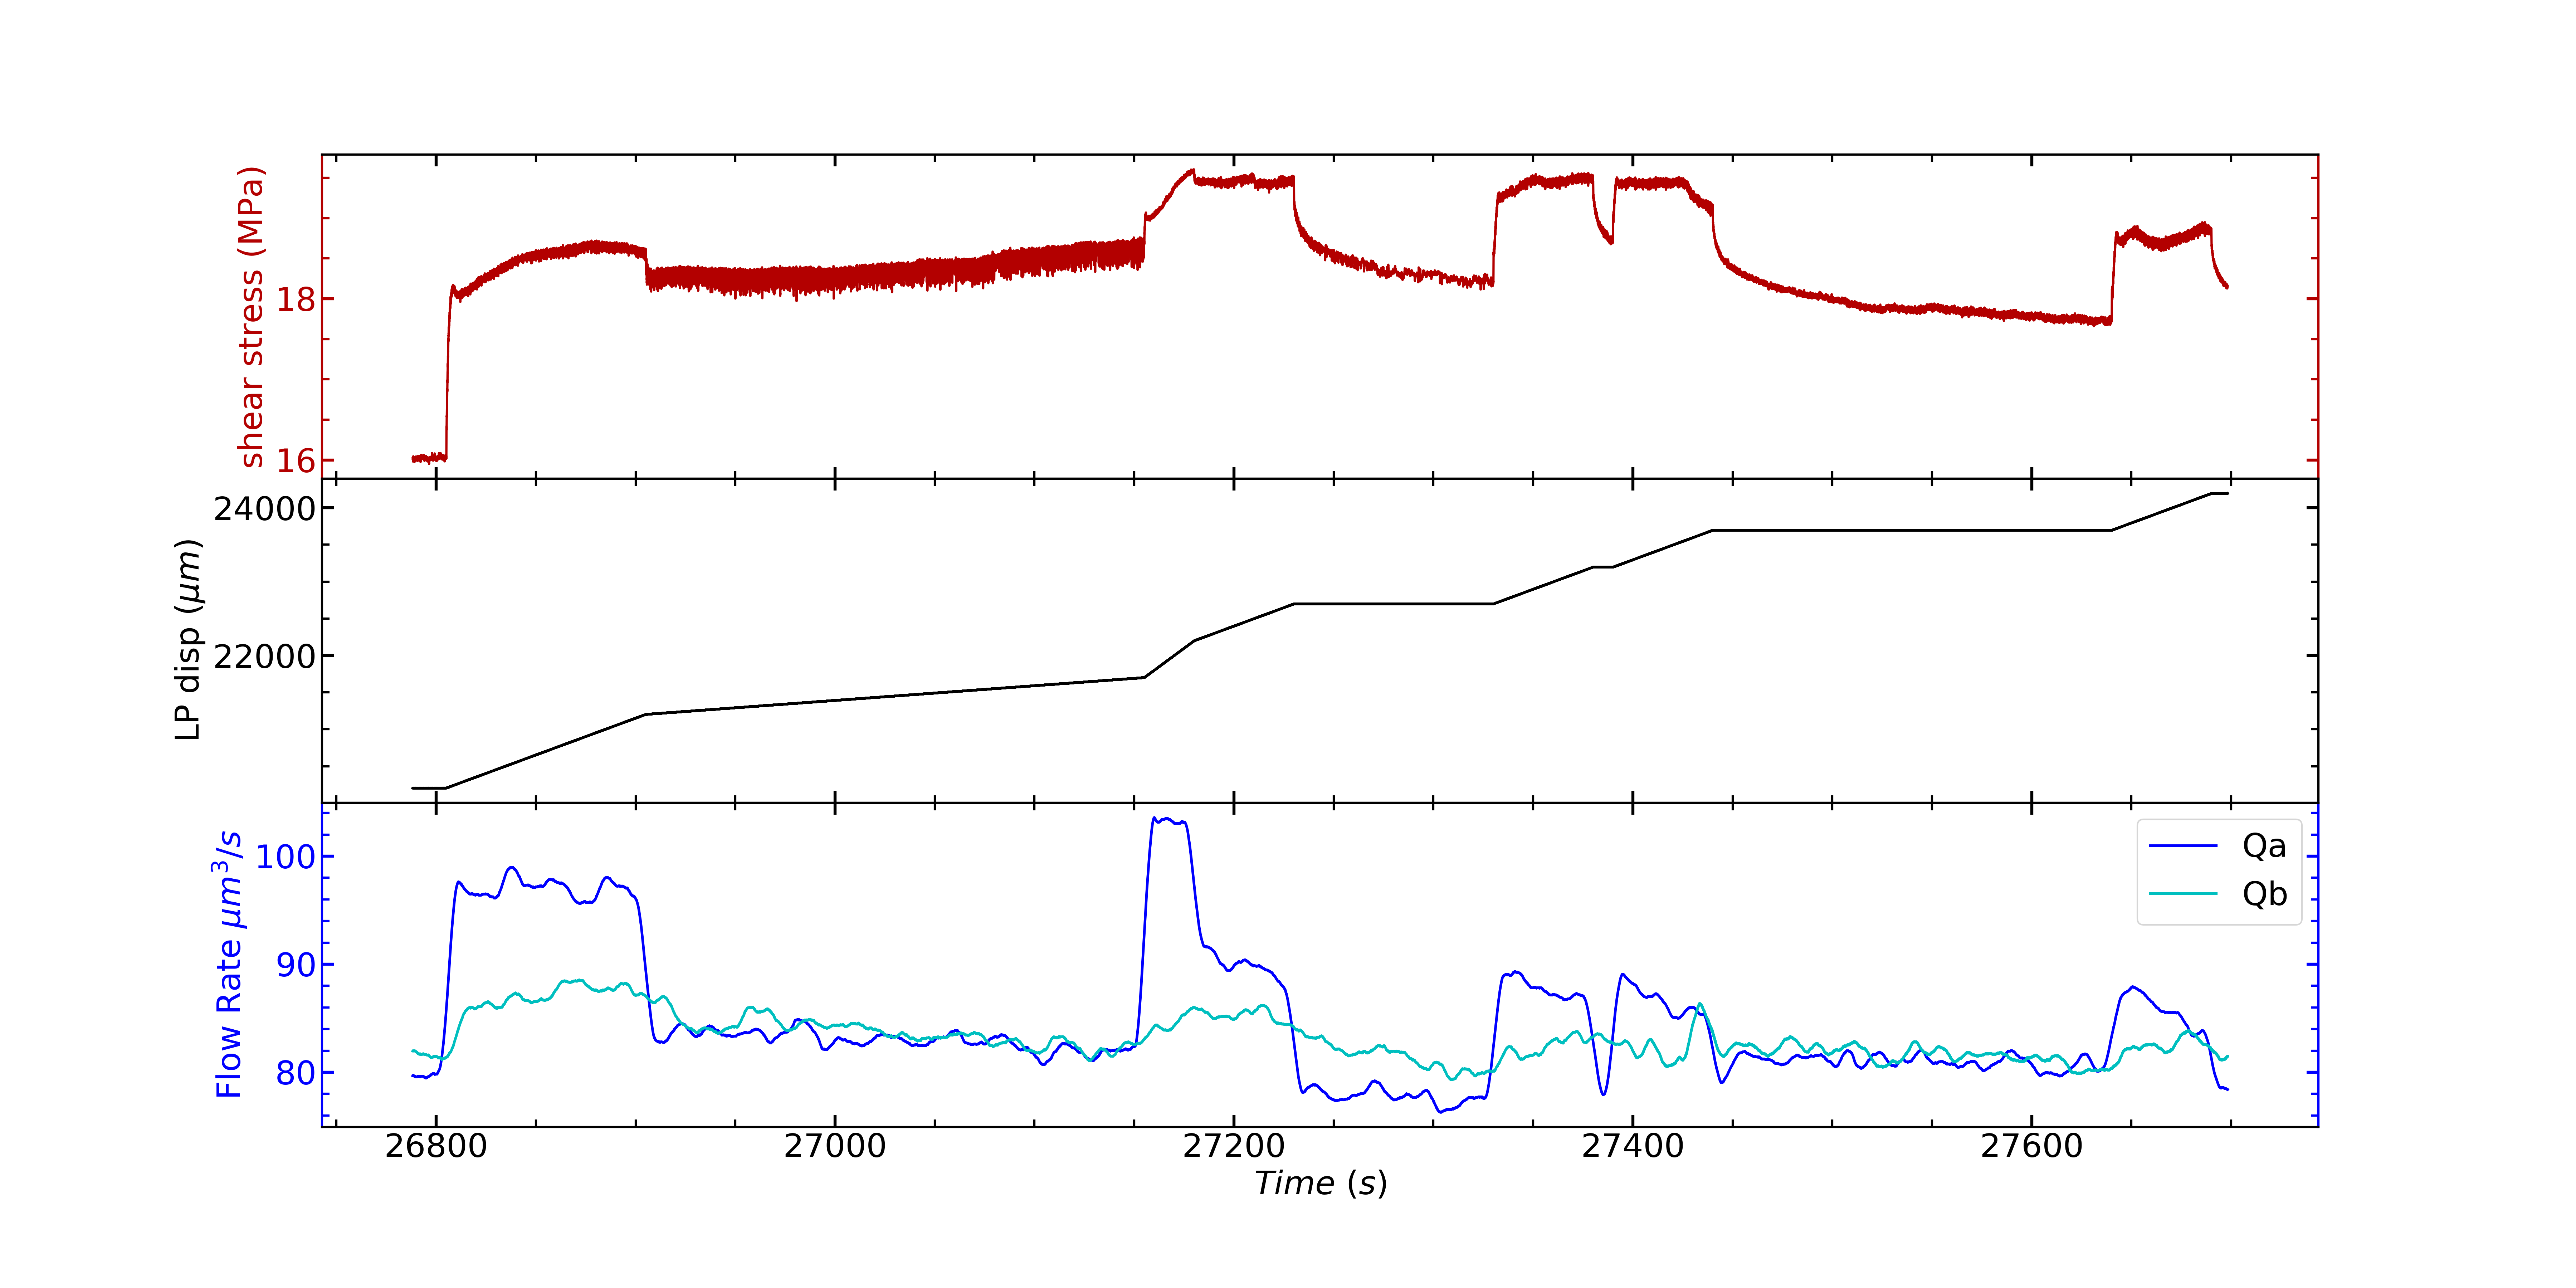
\includegraphics[width=1\columnwidth]{Shearing_p4975_shr2}
	\caption{Second shearing for p4975.}
	\label{fig:shr2_p4975}
\end{figure}

\clearpage


\begin{figure*}[ht]
	%\begin{sidewaysfigure}
	\centering
	%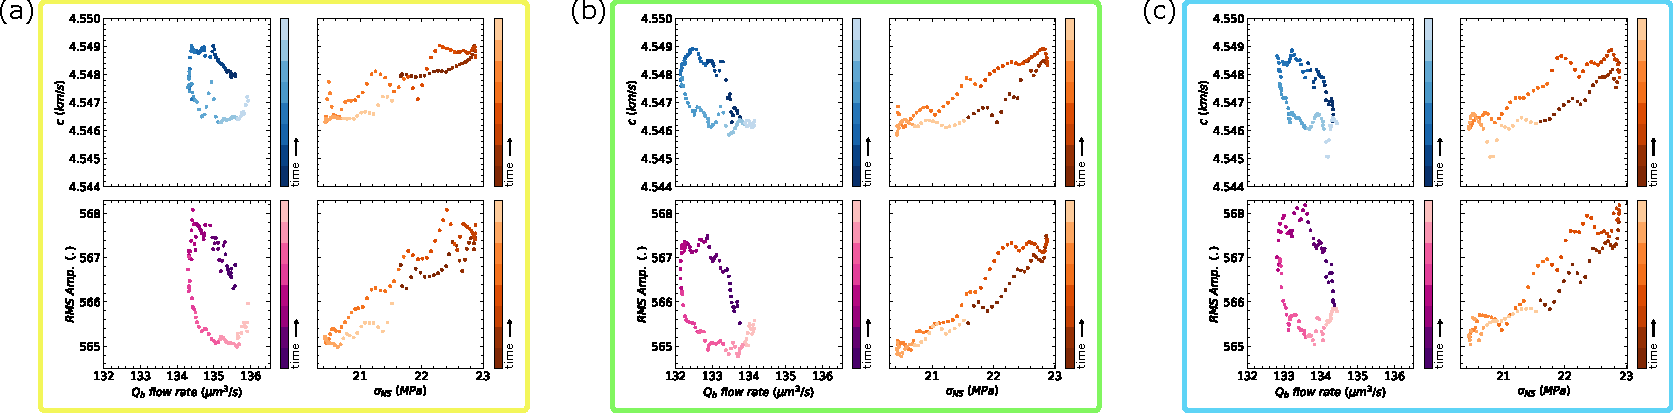
\includegraphics[width=0.9\columnwidth]{bowtie_p4975_run3b_01Hz_v3}
	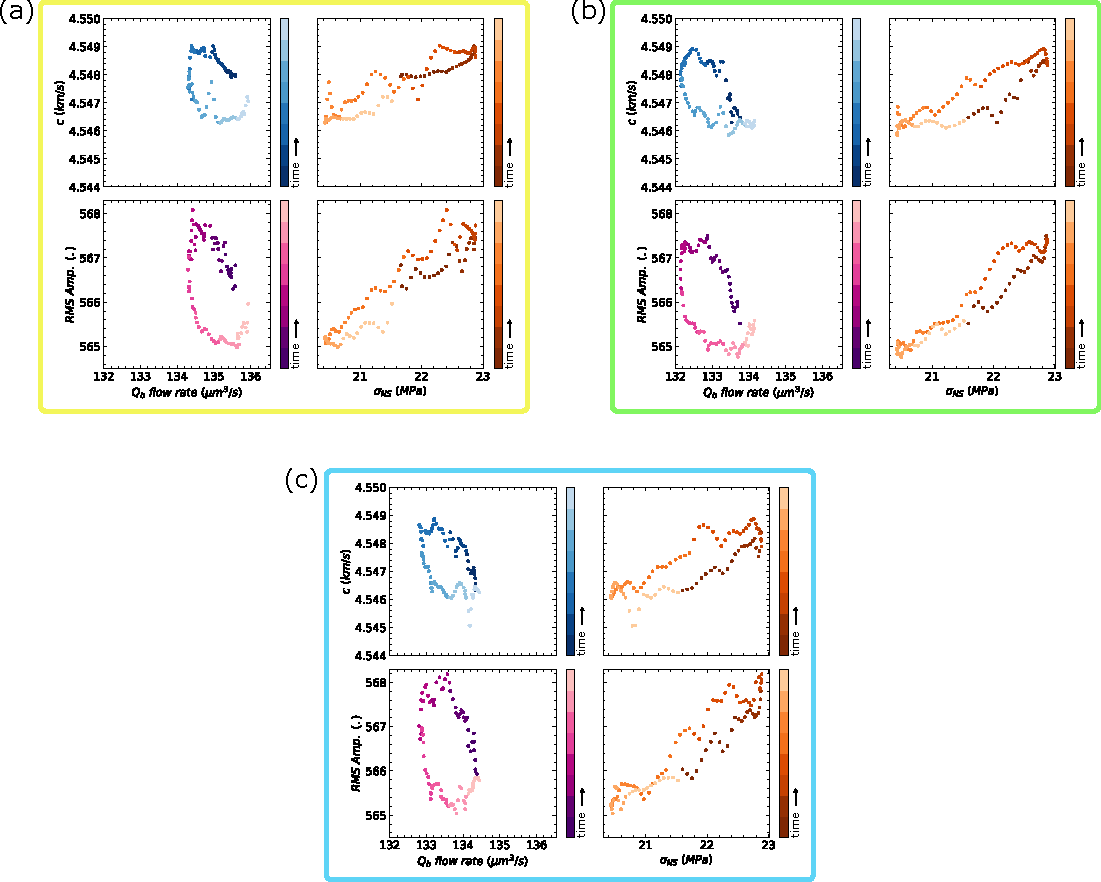
\includegraphics[width=0.9\columnwidth]{bowtie_p4975_run3b_01Hz_v3_portrait.pdf}
	\caption[]{Evolution of the fracture during a 1 MPa, 1 Hz normal stress oscillation during the first cycle (a), middle cycle (b), and last full cycle (c). The relationship between velocity and RMS Amplitude with outlet flow rate track each other throughout the oscillation, resulting in decreased flow.} %The point to make here is that the fracture is continuously changing -- the change in aperture results in change in velocity and flow paths.
	\label{fig:bowties}
\end{figure*}
%\end{sidewaysfigure}

The relationship between these parameters in the beginning, middle, and end of the oscillation are presented in Figure \ref{fig:bowties}. This figure also includes hysteresis plots that show how the wave velocity vary as a function of stress. Throughout this long oscillation the velocity-flow hysteresis loop generally evolves to a lower velocity and lower flow rate and the loop becomes slightly more closed. We also observe this general decrease in wave velocity as a function of applied stress throughout the history of the oscillation.If the oscillation persists long enough, the wave velocity modulations reach a steady-state. These observations demonstrate the magnitude of changes we are characterizing and also reinforce that the fracture is continuously evolving during the dynamic perturbations; contacts undergo compression and tension resulting in changing flow paths across the fracture.

\clearpage


\subsection{Nonlinear Elastodynamic Response: Relative Change in RMS Amplitude}
For elastic waves that travel across fractures the transmitted amplitude provides information on contact stiffness and area. Our data show that changes in RMS amplitude, $ \Delta A/ A_0 $, evolve in a similar manner to changes in p-wave velocity for both types of effective dynamic stressing (see Figure \ref{fig:delA_ns_amp}). In the post-fracture case p4975 results show that the change in transmitted p-wave amplitude becomes more negative with increasing normal stress amplitude; this trend is less obvious with pore pressure oscillation amplitude. Furthermore, there is little variation in these results with the order in which the oscillations were conducted. The situation is different for experiments p4966 in that the results are very scattered for normal stress oscillations and more coherent for pore pressure oscillations. The order of oscillation is most pronounced for oscillation amplitudes $ > 0.25 $ MPa, subsequent sets are less nonlinear. Surprisingly, normal stress oscillations in post-shear 1 of experiment p4966 produce positive changes in RMS amplitude, which contradict our findings with respect to $ \Delta c/c_0 $. Another interesting observation is that progressive shearing creates conditions that produce less nonlinearity. These differences are likely due to the complexity of fracture roughness and changes in contact stiffness with shear.

The averaged change in RMS as a function of $ \Delta k/k_0 $ is plotted in Figure \ref{fig:dela_plots2}. These plots show a complex relationship between the transmitted energy and fracture hydraulic properties. Normal stress oscillations of 40 Hz frequency consistently produce positive nonlinearity values. This and our observation that nonlinearity decreases with shearing are in fact physical rather than artifacts of data analysis, detailed in Section \ref{Supp}. Pore pressure oscillation results are more scattered but show a similar relationship as normal stress oscillations, but the underlying elasto-hydraulic mechanisms require further experimental investigation.

\clearpage

\begin{figure*}[ht]
	\centering
	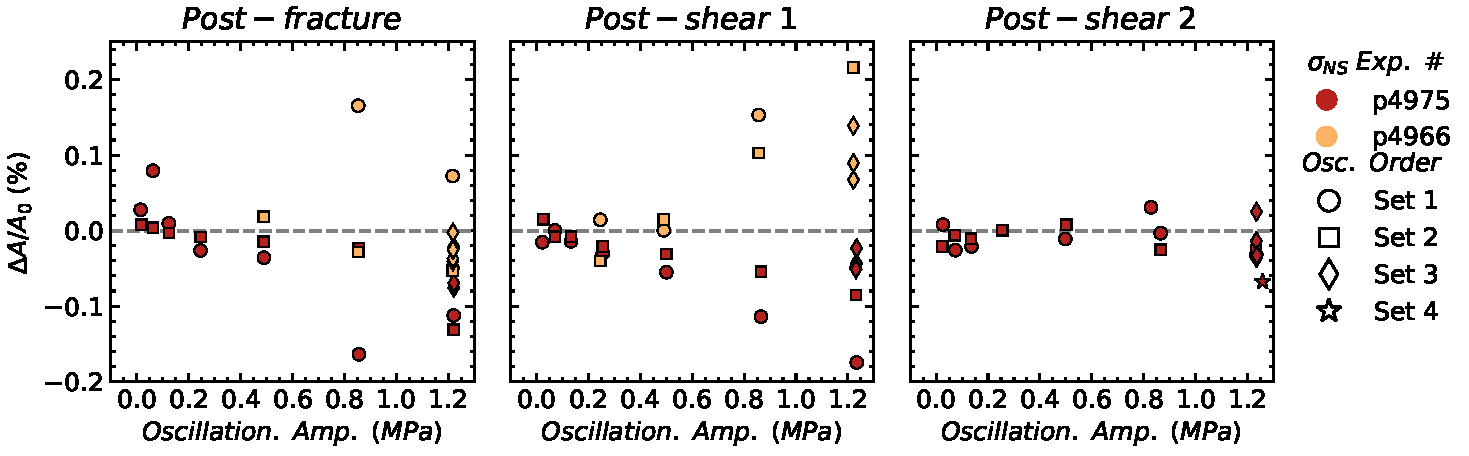
\includegraphics[width=1\columnwidth]{delA_amp_NS}
	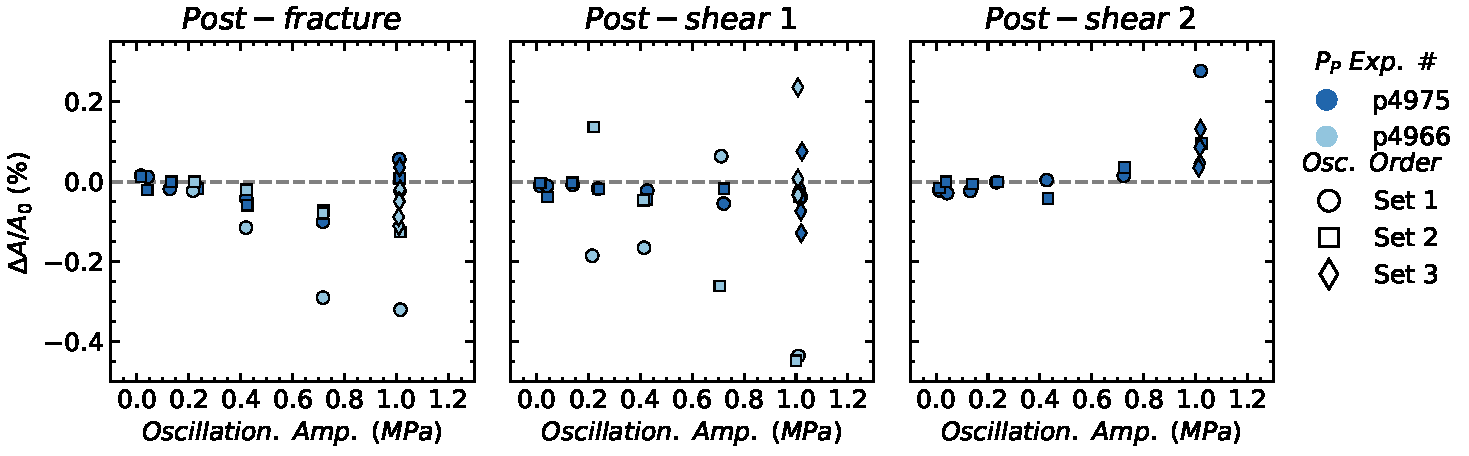
\includegraphics[width=1\columnwidth]{delA_amp_PP}
	%\enspace
	%\includegraphics[width=6cm]{post-frac_amp_array}
	\caption{RMS amplitude for direct-path receiver as a function of permeability change for $ \sigma_{NS} $ and $ P_P $ oscillations. Data point shapes oscillation order.  RMS amplitude decreases with oscillation amplitude and show little variation with order for experiment p4975. Order of oscillation is most pronounced for oscillation amplitudes $ > 0.25 $ MPa, Subsequent oscillation sets are less nonlinear; surprisingly, normal stress oscillations in post-shear 1 in p4966 produce positive changes in RMS amplitude. Furthermore, progressive shearing creates conditions that produce less nonlinearity, likely due to the complexity of fracture aperture and changes in contact stiffness. }
	\label{fig:delA_ns_amp}
\end{figure*}

\clearpage


\begin{figure*}[ht]
	\centering
	\includegraphics[width=1\columnwidth]{avg_DelA_perm_NS}
	\includegraphics[width=1\columnwidth]{avg_DelA_perm_PP}
	%\enspace
	%\includegraphics[width=6cm]{post-frac_amp_array}
	\caption{RMS amplitude averaged over all receivers as a function of permeability change for $ \sigma_{NS} $ and $ P_P $ oscillations. Data point shapes correspond to oscillation frequency and sizes to amplitude. There is a familiar trend that the average RMS amp. decreases with oscillation amplitude and frequency, except at high frequencies where there is anomalous behavior. Shearing the fracture weakens the relationship with relative permeability change.}
	\label{fig:dela_plots2}
\end{figure*}

\clearpage

\bibliography{biblio_d13}
\bibliographystyle{ieeetr}

\end{document}
